\chapter{Reverse engineering and binary analysis}

\section{Introduzione}
In questa parte degli appunti tratteremo di:
\begin{itemize}
    \item Come i programmi vengono compilati.
    \item Struttura di un file ELF.
    \item Deassemblamento di un file.
    \item Decompilazione di un file.
    \item Debug.
    \item Anti debug.
    \item Assembly.
    \item Kernel space vs user space.
    \item System call vs library call.
    \item Librerie dinamiche vs librerie statiche.
    \item Dynamic tracing.
\end{itemize}

\section{Linguaggio C}
Il reale problema del linguaggio \textit{C} è il comportamento degli errori. Per com'è strutturato gli errori lanciati dal linguaggio non sono specializzati, ciò è quello che cerchiamo quando ci troviamo ad analizzare un eseguibile perchè ci aiuterà nell'iniettare del codice arbitrario, questa problematica genera una \textbf{Nasal Demon} (comportamento indefinito).

\begin{ex}
    Per esempio facendo eseguire questo codice in C:
    \begin{lstlisting}[language=C]
        ...
        ++x + x++
        ...
    \end{lstlisting}
    otterremo così un nasal demons, in quanto verranno rilasciati risultati non deterministici.
\end{ex}

\subsection{Come viene compilato un programma}

Supponiamo di avere del codice C come questo:
\begin{lstlisting}[language=C]
    #include <stdio.h>
    
    int main (int argc, char** argv ) { 
        char who[] = world;
        print ("Hello %s! \n", who);
        return 0 ;
    }
\end{lstlisting}
\textbf{Domanda:} Quali sono i passaggi per effettuare la compilazione?

\subsubsection{Precompilazione}
Il compilatore è istruito per includere codice o tradurre codice da altri sorgenti. Perciò il contenuto delle librerie (e.g. stdio.h) sarà inserito in testa al \textit{main} del programma.

\subsubsection{Compilazione}
Una volta passato per il precompilatore il passo successivo sarà effettuato dal compilatore che si occuperà di tradurre il codice \textit{C} in codice \textit{assembly}.

\begin{lstlisting}[language={[x86masm]Assembler}]
main:
    .LFB0:
    .cfi_startproc
    pushq %rbp
    .cfi_def_cfa_offset 16
    .cfi_offset 6, -16
    movq %rsp , %rbp
    . cfi_def_cfa_register 6
    subq $16 , %r s p
    movl %edi , -4(%rbp )
    movq %r s i , -16(%rbp )
    leaq .LC0(%rip), %rdi
    call puts@PLT
    movl $0 , %eax
    leave
    .cfi_def_cfa 7, 8
\end{lstlisting}

\subsubsection{Assembly}
In questa fase il codice assembly ottimizzato verrà tradotto in \textbf{opcode}, linguaggio binario comprensibile dalla macchina, mediante un assembler.
\begin{lstlisting}[language=bash]
    command:
    file test.o

    output:
    test.o: ELF 64-bit LSB relocatable, x86-64, version 1 (SYSV), not stripped 
\end{lstlisting}

\subsubsection{Linking}
Se dovessimo aprire il codice potremmo vedere come le nostre chiamate alle funzioni siano dei \textit{placeholder} e non il codice della funzione scritta in \textit{C}, questo codice sarà iniettato a livello nel programma dal \textit{linker (ld)}.

\subsection{Struttura di un file ELF}
Il binario che avremo come risultato dopo tutti i passaggi sarà serializzato in un file strutturato e formattato in formato \textbf{ELF (Executable and Linkable Format)}.
Questo formato dichiara differenti aree chiamate segmenti:
\begin{lstlisting}[language=bash]
    command:
    readelf -S $(which /bin/ls)
\end{lstlisting}

\begin{figure}[h!]
    \centering
    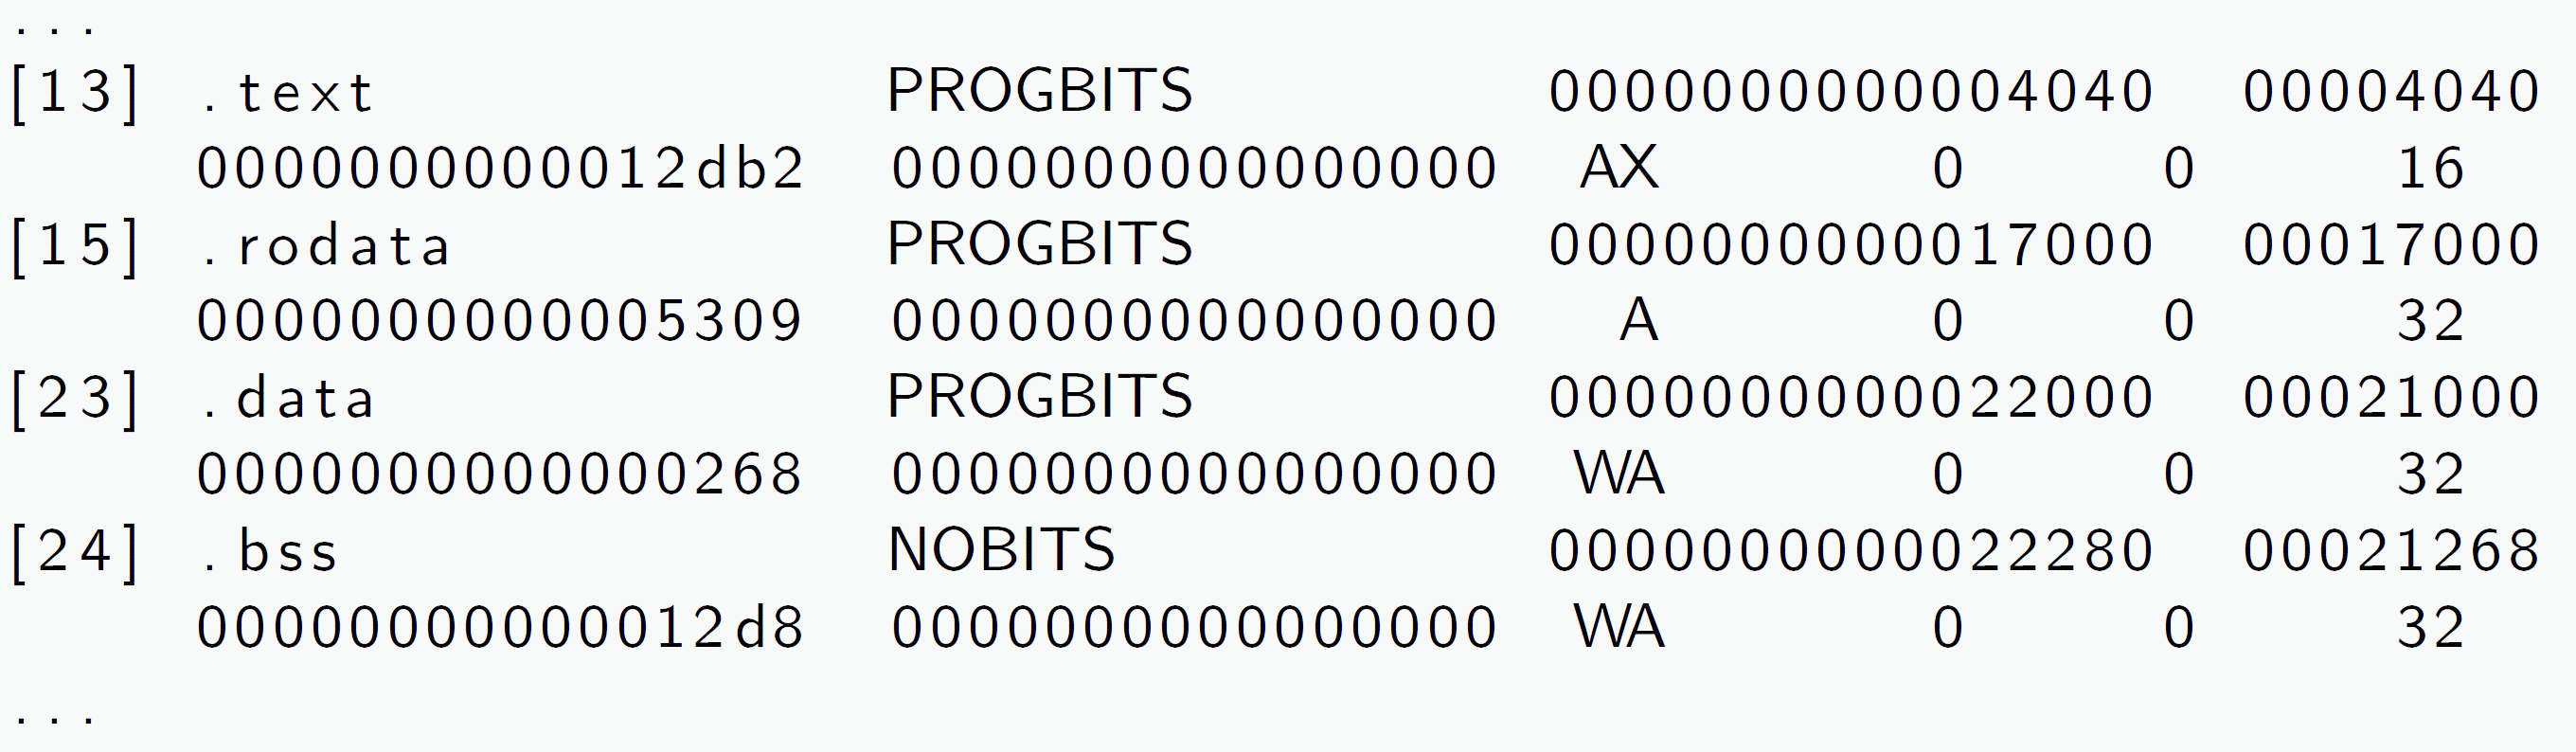
\includegraphics[width=.6\linewidth]{res/ELF_Structure.png}
    \caption{}
\end{figure}
Alcuni dei segmenti più comuni sono i seguenti:
\begin{itemize}
    \item \textbf{.interp}, contiene il percorso dell'interprete che sarà utilizato per eseguire il programma;
    \item \textbf{.text}, contiene il codice dell'eseguibile (e.g. return 3+4);
    \item \textbf{.rodata}, contiene i dati in sola lettura (e.g. printf("ciao"));
    \item \textbf{.data}, contiene i dati sia in lettura sia in scrittura (e.g. int x = 0x41);
    \item \textbf{.bss}, contiene le variabili globali non ancora inizializzate (e.g. static int x).
\end{itemize}
Verranno introdotti altri segmenti successivamente utili per la sicurezza o per gli exploit.

\subsubsection{Information Leak}
Uno dei problemi del linguaggio \textit{C} è l'information leakage in quanto tutte le variabili non vengono tradotte dal compilatore ma rimangono in chiaro nel codice, ciò permette di vederle anche dal codice compilato. Sopponiamo di avere il seguente codice sorgente:
\begin{lstlisting}[language=C]
    #include <stdio.h>
    #include <string.h>

    int main (int argc, char** argv) {
        char *password = "super-secret-password"
        if (argc < 2) {
            printf("Usage : %s <name>\n" , argv [0]);
            return 1;
        }

        if (!strcmp(password, argv[1])) {
            print("Access granted!\n");
        }
        return 0;
    }
\end{lstlisting}
Effettuando una ricerca nel file compilato potremo vedere come la variabile inizializzata con la nostra password saraà in chiaro.
\begin{lstlisting}[language=bash]
    command:
    strings test | grep pass

    output:
    super-secret-password
\end{lstlisting}

\section{Analisi dei file compilati}

Invertendo il processo di compilazione saremo in grado di tornare al codice assembly del programma. La parte più difficile però sarà passare dal codice assembly al codice in \textit{C}, in quanto al contrario del codice assembly che è 1:1 con l'opcode, il codice in \textit{C} non lo è con l'assembly del programma.
Questo perchè essendo un linguaggio a più alto livello avrà dettagli implementativi che ne possono modificare il reverse.
Per questo si utilizzano varie tecniche per fare il reverse da codice assembly a codice \textit{C}:
\begin{itemize}
    \item \textbf{Static analysis}, analisi del codice senza mandarlo in esecuzione;
    \item \textbf{Dynamic analysis}, analisi del codice attraverso l'esecuzione dello stesso.
\end{itemize}

\subsection{Static Analysis}
L'analisi statica come detto in precedenza si effettua sul compilato stesso senza andarne ad analizzare i comportamenti durante l'esecuzione.

\subsubsection{Disassembly}
La fase di assembly è facilmente reversibile, si effettua andando a mappare l'opcode del programma con l'equivalente in linguaggio X86\_64. Siccome l'assembly X86\_64 non utilizza un particolare alfabeto per i dati e per il codice, si potrà disassemblare anche il garbage (e.g. disassemblando .rodata o .data).
Uno dei tool di più facile utilizzo ma anche poco potente utilizzabile è \textit{objdump}.

Supponiamo di voler vedere il codice assembly del file sorgente precedentemente visto:
\begin{lstlisting}[language=bash]
    command:
    objdump -D ./test | grep '^[0-9]\+ <main>' -A 10
\end{lstlisting}

Otterremo un output del genere:
\begin{figure}[h!]
    \centering
    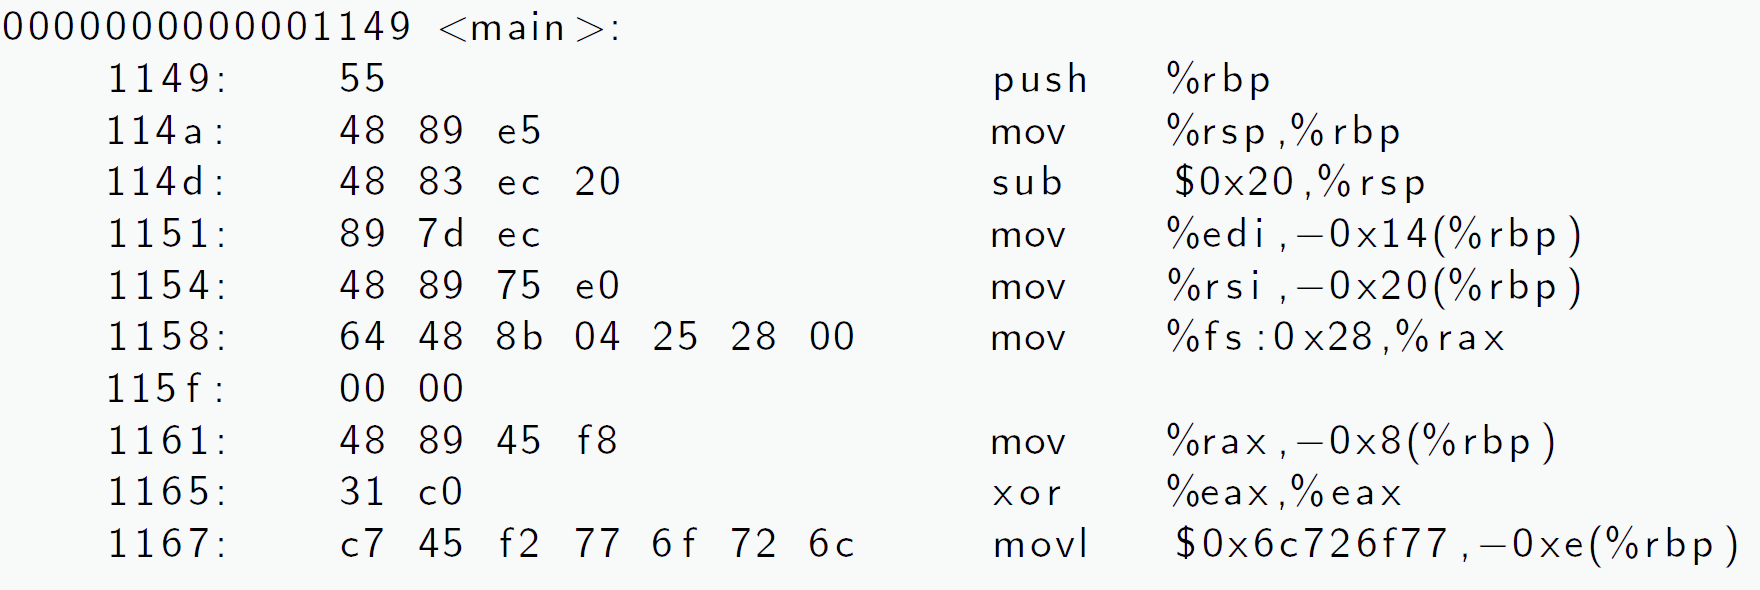
\includegraphics[width=.6\linewidth]{res/objdump_1.png}
    \caption{}
\end{figure}

Come possiamo vedere avremo come output l'intero codice assembly generato dall'opcode precedente.
Per svolgere il reverse engineering dell'opcode esistono diverse tecniche che si possono utilizzare:
\begin{itemize}
    \item \textbf{Linear sweep};
    \item \textbf{Recursive descent};
    \item \textbf{FLIRT (Fast Library Indication and Recognition Technology)}, una combianzione delle precedenti.
\end{itemize}

Un disassembler linear sweep analizza il codice partendo dalla prima riga fino ad arrivare all'ultima analizzandolo byte per byte, questo però può portare ad avere delle sequenza di codice errate nel caso in cui i dati sono mischiati con il codice o nel caso di salti all'interno porterebbe a non tradurre le istruzioni successive.
Al contrario un disassembler recursive descent analizza il codice basandosi sul \textbf{CFG (Control Flow Graph)} del binario, ciò gli permette di tradurre tutto il codice superando i limiti del precedente, questo metodo però risulta spesso difficoltoso quando nel codice sono presenti chiamate indirette che dipendono dal contenuto dei registri o posizioni di memoria.
\clearpage
\subsection{Decompilation}
Una volta dissassemblato l'opcode potremo effettuare la decompilazione, che porterà ad avere un codice \textbf{C-like}, in questo caso il codice generato potrà essere abbastanza diverso dal sorgente vero e proprio in quanto una volta compilato il sorgente perderà tutti i commenti e cambierà i nomi delle variabili, ciò porterà ad una difficolta da parte dell'analista nel comprendere il codice decompilato.
\begin{figure}[h!]
    \centering
    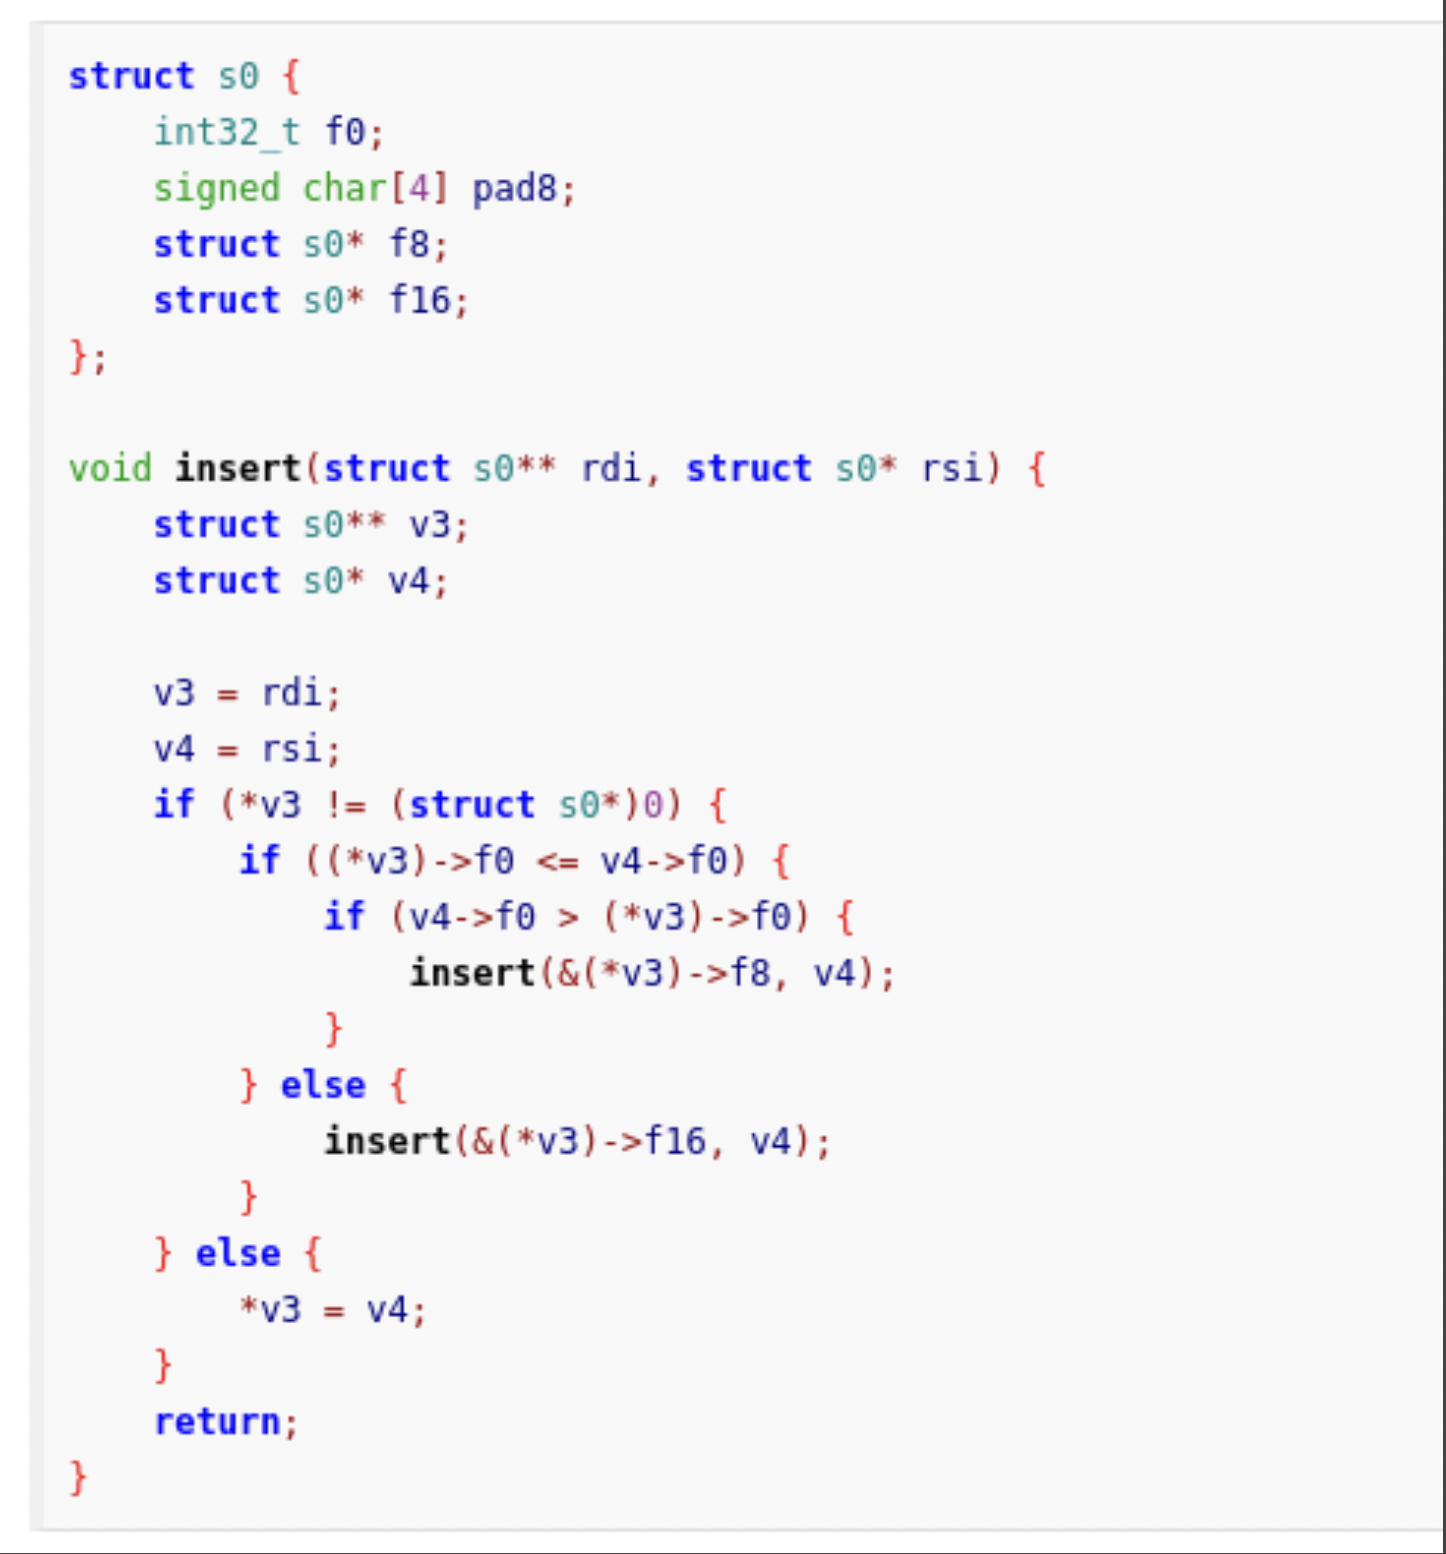
\includegraphics[width=.6\linewidth]{res/decompiled_code.png}
    \caption{}
\end{figure}

\subsubsection{Anti static analysis technique}
I disassembler statici spesso sono compelssi e la maggior parte delle volte utilizzano tecniche euristiche e approcci complessi per l'analisi del codice.
Un esempio di tecnica anti debug può essere effettuata modificando gli headers cercati da objdump in modo tale da non far funzionare il software. Un altro approccio è offuscare il codice inserendo istruzioni inutili o ottimizzazioni "strane" in modo da rendere più difficoltosa l'analisi dai software.
Un esempio è quello che segue:
\begin{figure}[h!]
    \centering
    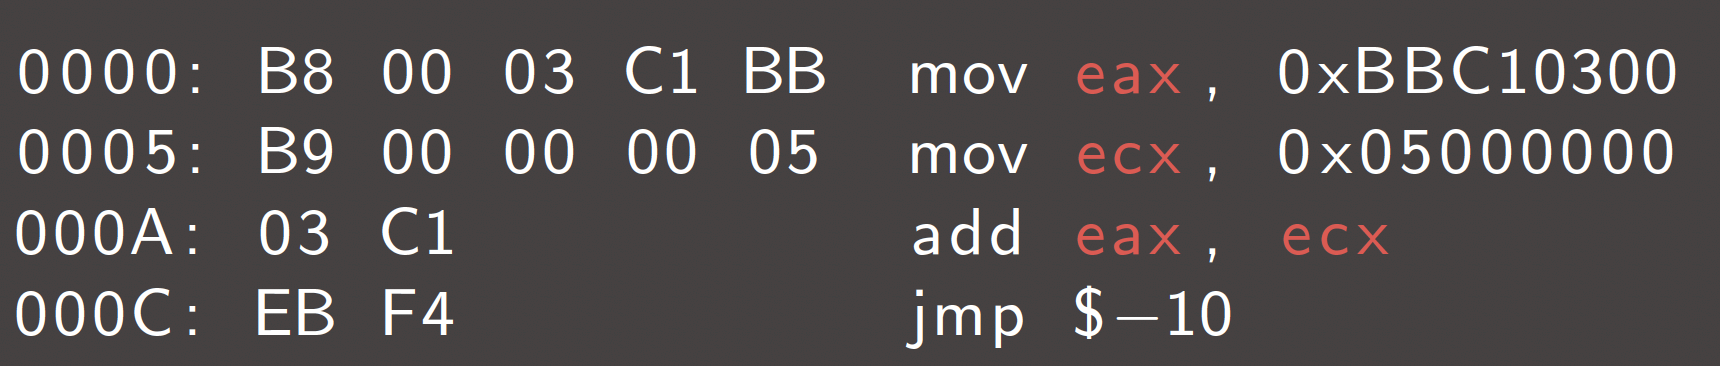
\includegraphics[width=.6\linewidth]{res/obfuscated_code.png}
    \caption{Disassembly dell'opcode partendo dall'indirizzo 0x00}
\end{figure}

\begin{figure}[h!]
    \centering
    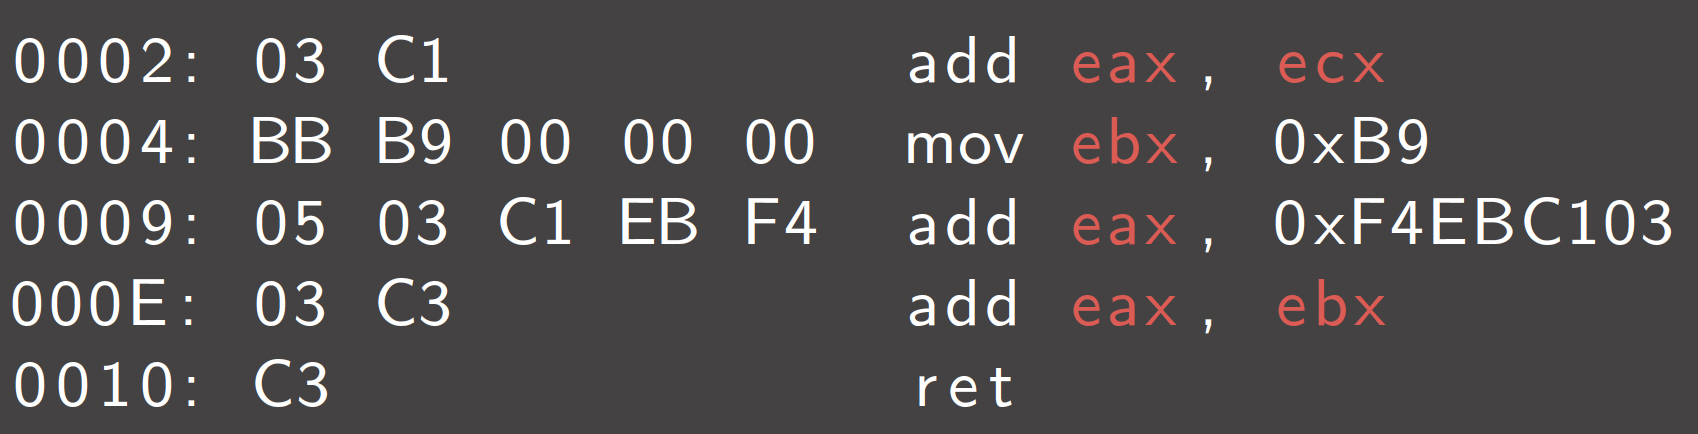
\includegraphics[width=.6\linewidth]{res/obfuscated_code2.png}
    \caption{Disassembly dell'opcode partendo dall'indirizzo 0x02}
\end{figure}
Come si può vedere partendo ad analizzare il codice da un altro punto avremo un risultato totamente diverso, ciò renderà l'analisi più difficoltosa.
\clearpage
\section{Com'è composta la memoria}

\subsection{Stack}
\begin{wrapfigure}{r}{0.5\textwidth}
    \begin{center}
        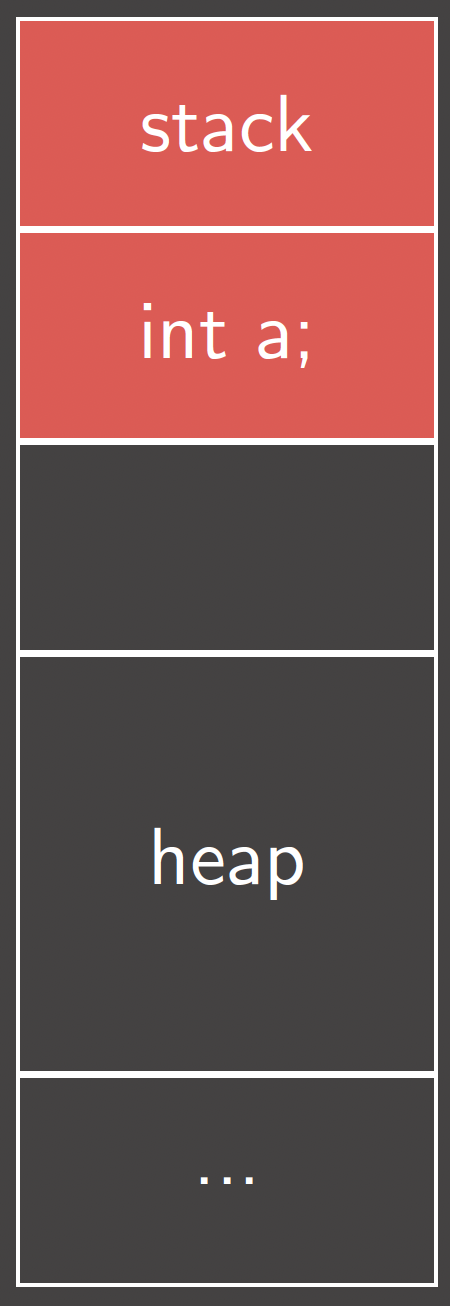
\includegraphics[width=0.1\textwidth]{res/stack.png}
        \caption{Raffigurazione dello stack}
    \end{center}
\end{wrapfigure}
Lo \textbf{Stack} è la porzione di memoria dove risiedono tutti i dati di un programma, quando chiami una funzione o dichiari una variabile esse verranno posizionate nello stack, essa è gestita automaticamente dal sistema.
Lo stack cresce in verso il basso, cioé verso gli indirizzi di memoria minori.

\subsection{Heap}
\begin{wrapfigure}{l}{0.5\textwidth}
    \begin{center}
        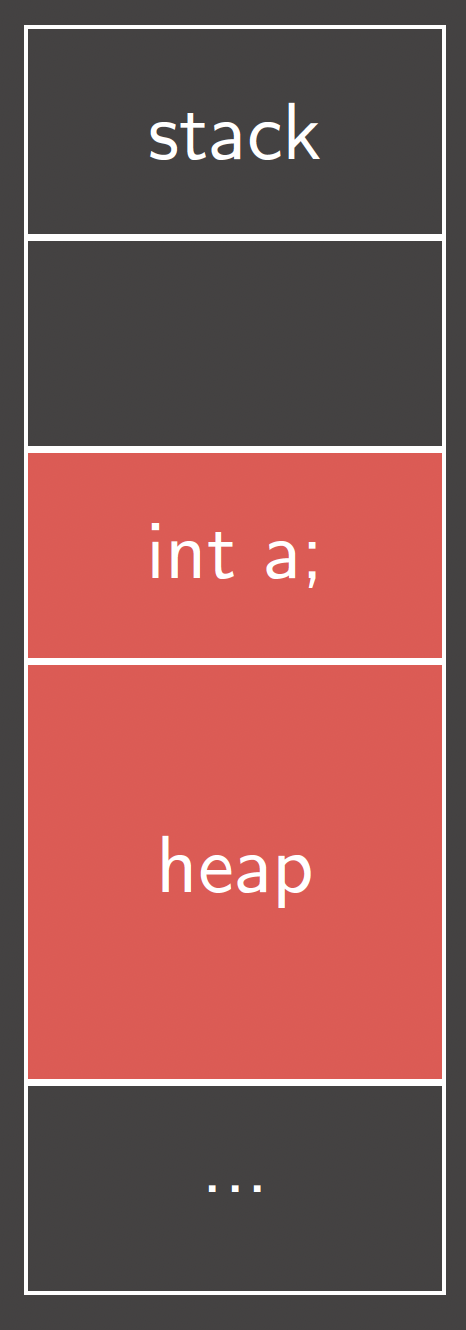
\includegraphics[width=0.1\textwidth]{res/heap.png}
        \caption{Raffigurazione dell'heap}
    \end{center}
\end{wrapfigure}
La memoria \textbf{Heap} al contrario dello stack non viene gestita dal sistema ma è compito del programmatore attraverso le corrette chiamate alle funzioni (e.g. malloc o delete in C), essa è utilizzata per distribuire il possesso di limitate quantità di memoria tra varie porzioni di dati e codice.

\clearpage
\subsection{Protezione per la memoria}
Al giorno d'oggi i processori implementano vari sistemi di protezione della memoria, infatti essa non sarà mai accessibile direttamente da un processo ma verrà demandato il controllo alla \textbf{MMU} che si occuperà di prelevare e rimuovere i vari dati e le istruzioni dalla memoria e a prevenire eventuali errori di segmentation fault.
\begin{figure}[h!]
    \centering
    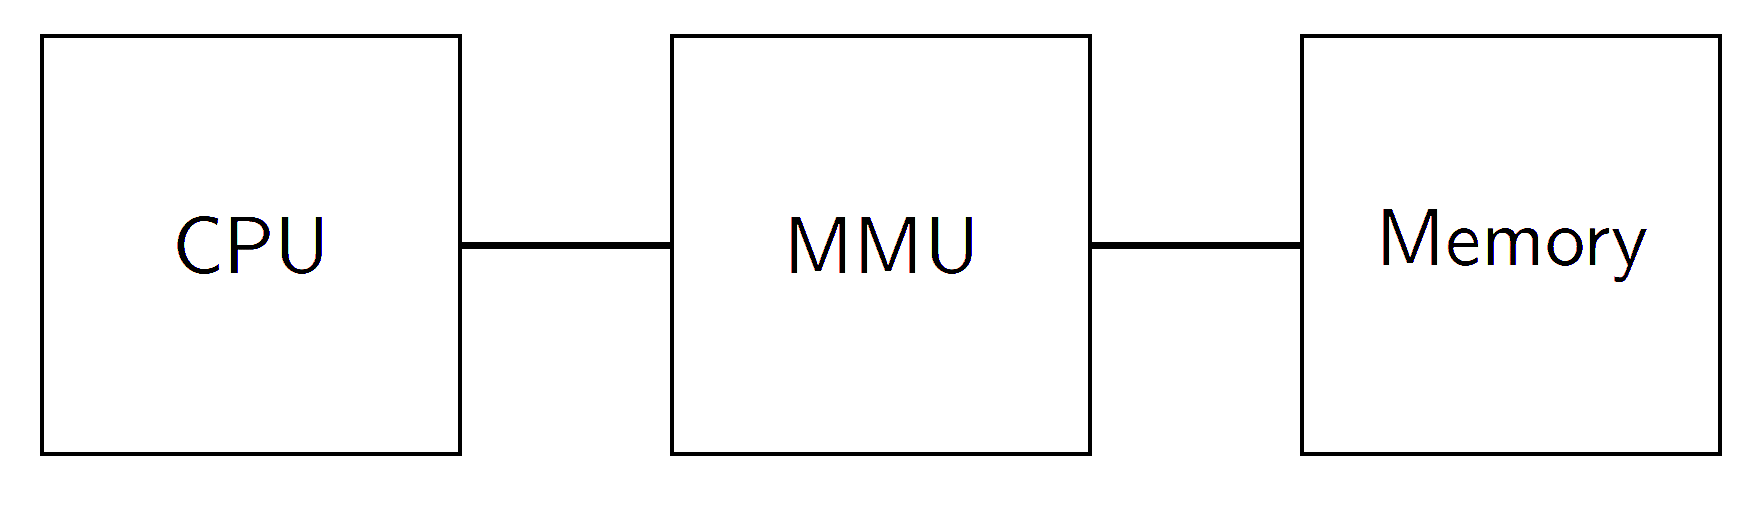
\includegraphics[width=.4\linewidth]{res/MMU.png}
    \caption{}
\end{figure}

Ciò ha portato anche all'implementazione di vari livelli di permessi per una processo, essi prendono il nome di \textbf{Ring}, permettono di isolare la memoria evitando una manipolazione errata della stessa.
\begin{figure}[h!]
    \centering
    
\includegraphics[width=.5\linewidth]{res/Ring.png}
    \caption{}
\end{figure}

Questi anelli sono nuimerati da 0 a 3, con 0 l'anello più privilegiato e 3 il meno:
\begin{itemize}
    \item \textbf{Ring 0}, è il ring dove viene eseguito il sistema operativo e da accesso ai privilegi massimi (kernel mode);
    \item \textbf{Ring 1}, generalmente poco utilizzato;
    \item \textbf{Ring 2}, anch'esso generalmente poco utilizzato;
    \item \textbf{Ring 3}, utilizzato per i permessi a livello applicativo.
\end{itemize}
Alcune implementazioni possono avere ulteriori due ring:
\begin{itemize}
    \item \textbf{Ring -1}, assegnato all'hypervisor delle macchine virtuali;
    \item \textbf{Ring -2}, assegnato al bios manager.
\end{itemize}

\section{Registri General Purpose}
Il processore x86-64 ha 16 registri general purpose:
\begin{center}
    \begin{table}[]
        \centering
        \begin{tabular}{|c|c|c|c|c|c|c|c|}
            ax & bx & cx & dx & si & di \\
            sp & bp \\
            r8 & r9 & r10 & r11 & r12 & r13 & r14 & r15
        \end{tabular}
        \caption{Esempio filesystem Linux}
    \end{table}
\end{center}
Essendo stato afflitto da varie patch questi registri sono stati resi accessibili non solo in modalità 64 bit ma anche 32, 16 e 8 bit:
\begin{itemize}
    \item \textbf{full register}, 64 bit (e.g. \textit{rax});
    \item \textbf{half register}, 32 bit (e.g. \textit{eax});
    \item \textbf{$\frac{1}{4}$ register}, 16 bit (e.g. \textit{ax});
    \item \textbf{$\frac{1}{8}$ register}, 8 bit (e.g. \textit{al}).
\end{itemize}

Esistono anche alcuni registri speciali che sono automaticamente utilizzati dalla CPU, essi sono:
\begin{itemize}
    \item \textbf{rip}, puntatore all'istruzione che deve essere eseguita nel successivo passaggio;
    \item \textbf{rsp}, usata automaticamente per salvare il puntatore dello stack frame con push e pop;
    \item \textbf{rflags}, descrive lo stato dell'esecuzione corrente (e.g. lo zero indica che l'istruzione precedente ha ritornato 0);
    \item \textbf{rbp}, non usata automaticamente dalla CPU ma normalmente serve a calcolare l'offset dalla memory location;
\end{itemize}

Esistono altri registri a supporto della CPU chiamati \textbf{xmm0} a \textbf{xmm15} abilitati per operazioni \textbf{SIMD register (Single Instruction Multiple Data)}, servono ad accelerare le operazioni di crittografia o di grafica vettoriale, generalmente da 128 o 256 bit:
\begin{itemize}
    \item \textbf{AESENC xmm1,xmm2/m128}, esegue un round di AES Encryption Flow round key partendo dal secondo operando, utilizzando il dato da 128bibt (stato) dal primo operando e salva il risultato nell'operando di destinazione;
    \item \textbf{AESENCLAST xmm1, xmm2/m128}, esegue le analoghe operazioni del caso precendente ma eseguendo l'ultimo round;
    \item \textbf{AESKEYGENASSIST xmm1, xmm2/m128}, assiste l'espansione del cipher key AES, calcolando gli step fino
\end{itemize}
\begin{ex}
    Supponiamo di avere il seguente codice assembly per una macchina x86\_64:
    \begin{figure}[h!]
        \centering
        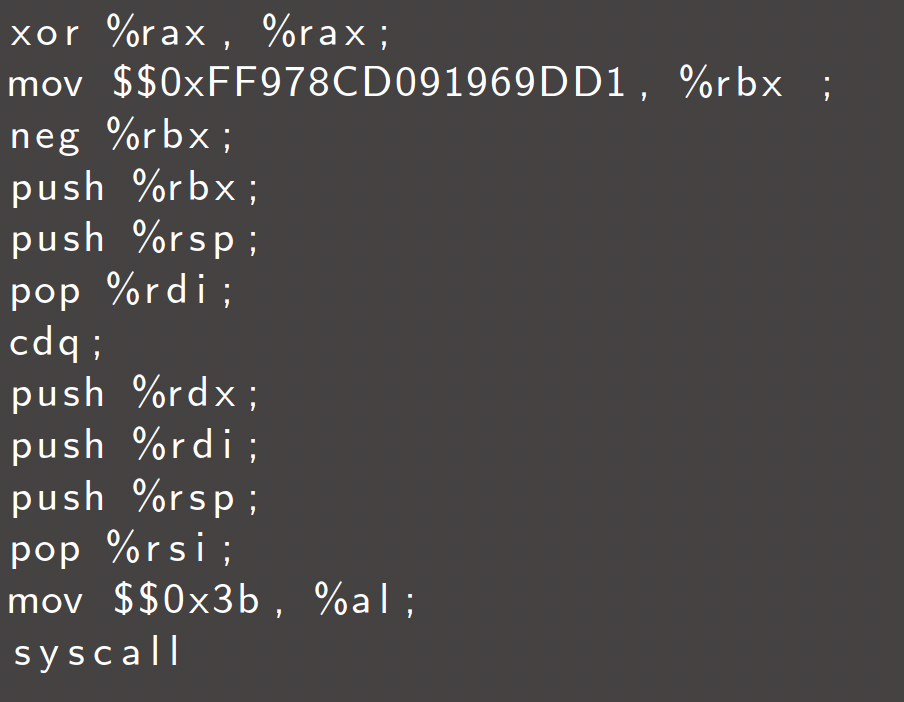
\includegraphics[width=.4\linewidth]{res/example_x86_code.png}
        \caption{}
    \end{figure}
    \\
    Come possiamo vedere la riga di codice più significativa è: 
    \begin{lstlisting}[language={[x86masm]Assembler}]
        mov $$0xFF978CD091969DD1, %rbx;
    \end{lstlisting}
    La prima cosa che dovremmo chiederci è: cosa vuol dire quel valore?
    Possiamo notare come nella riga successiva si vada a effettuare un \textit{not bitwise} e successivamente un complemento a 2 su quel registro.
    \begin{lstlisting}[language={[x86masm]Assembler}]
        neg %rbx;
    \end{lstlisting}
    Ciò porta a salvare nel registro la seguente string: \textbf{.bin/sh}, come possiamo vedere questo codice cercherà di aprire una shell e questo ci darà la possibilità di accedere al sistema infettato.
    Una volta manipolati i vari registri un pò anche per camuffare il codice possiamo veder ecome verrà richiesta una \textit{syscall} che alzerà la richiesta al sistema operativo per eseguirla, dandoci a questo punto il pieno accesso a una shell di sistema.
\end{ex}

\begin{ex}
    Un altro esempio lo possiamo vedere con questo codice: 
    \begin{figure}[h!]
        \centering
        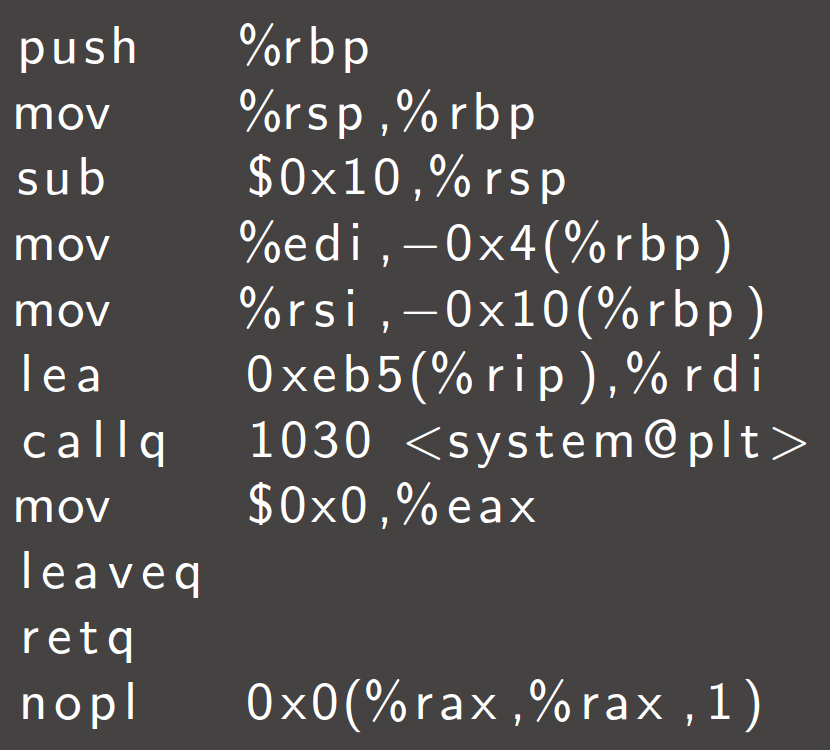
\includegraphics[width=.4\linewidth]{res/example_x86_code2.png}
        \caption{}
    \end{figure}
    Come possiamo vedere, nella seguente riga verrà chiamata una shell di sistema utilizzando una chiamata di libreria (system).
    \begin{lstlisting}[language={[x86masm]Assembler}]
        callq 1030 <system@plt>
    \end{lstlisting}
\end{ex}

\subsection{Dynamic analysis}
Un altro tipo di analisi citita in precedenza è l'analisi dinamica, essa viene effettuata eseguendo il codice e analizzandolo a runtime.
Per effettuare questo tipo di analisi si utilizzano i debugger come \textit{GDB} che permette di viasualizzare e analizzare le istruzioni che sono in esecuzione.
Una tenica per mitigare questo tipo di analisi è utilizzare un cronometro in modo tale da bloccare il debugger.

\subsubsection{GDB}
Alcuni esempi di comandi di \textit{GDB} sono:
\begin{itemize}
    \item \textbf{r < <(shell command)}, esegue il programma con input da una shell script, come se fosse una pipe;
    \item \textbf{ni}, passa alla prossima istruzione;
    \item \textbf{si}, salta dentro il jump
    \item \textbf{info register}, stampa lo stato dei registri in quell'istante;
    \item \textbf{b printf}, invoca un breakpoint all'invocazione di una printf;
    \item \textbf{b *0x123456}, invoca un breakpoint all'indirizzo richiesto;
    \item \textbf{d3}, elimina il breakpoint numero 3. 
\end{itemize}
GDB, e in genere tutti i debugger su linux, per tracciare l'esecuzione di un processo invocano la systemcall \textit{ptrace}, che si occupa di tracciare il processo e recuperare i valori dei registri nello stato corrente.

Tra le possibilità di GDB vi sono anche quelle di modificare i registri e le righe di codice del processo.
\textbf{Domanda:} Cosa successe se a un processo in esecuzione su GDB gli attacco un processo privilegiato, e un esecuzione privilegiata (e.g. setuid)?
GDB si occuperà di rimuovere i privilegi prima di eseguire il codice in modalità debug ciò permette di non modificare i registri. Il debug è uno dei primi motivi di inconsistenza.

\subsection{Library}
Una libreira è un insieme di funzioni composta da simboli che che permettono di collegare altre applicazioni.
\begin{lstlisting}[language=bash]
    nm /lib64/libasan.so
\end{lstlisting}
\begin{figure}[h!]
    \centering
    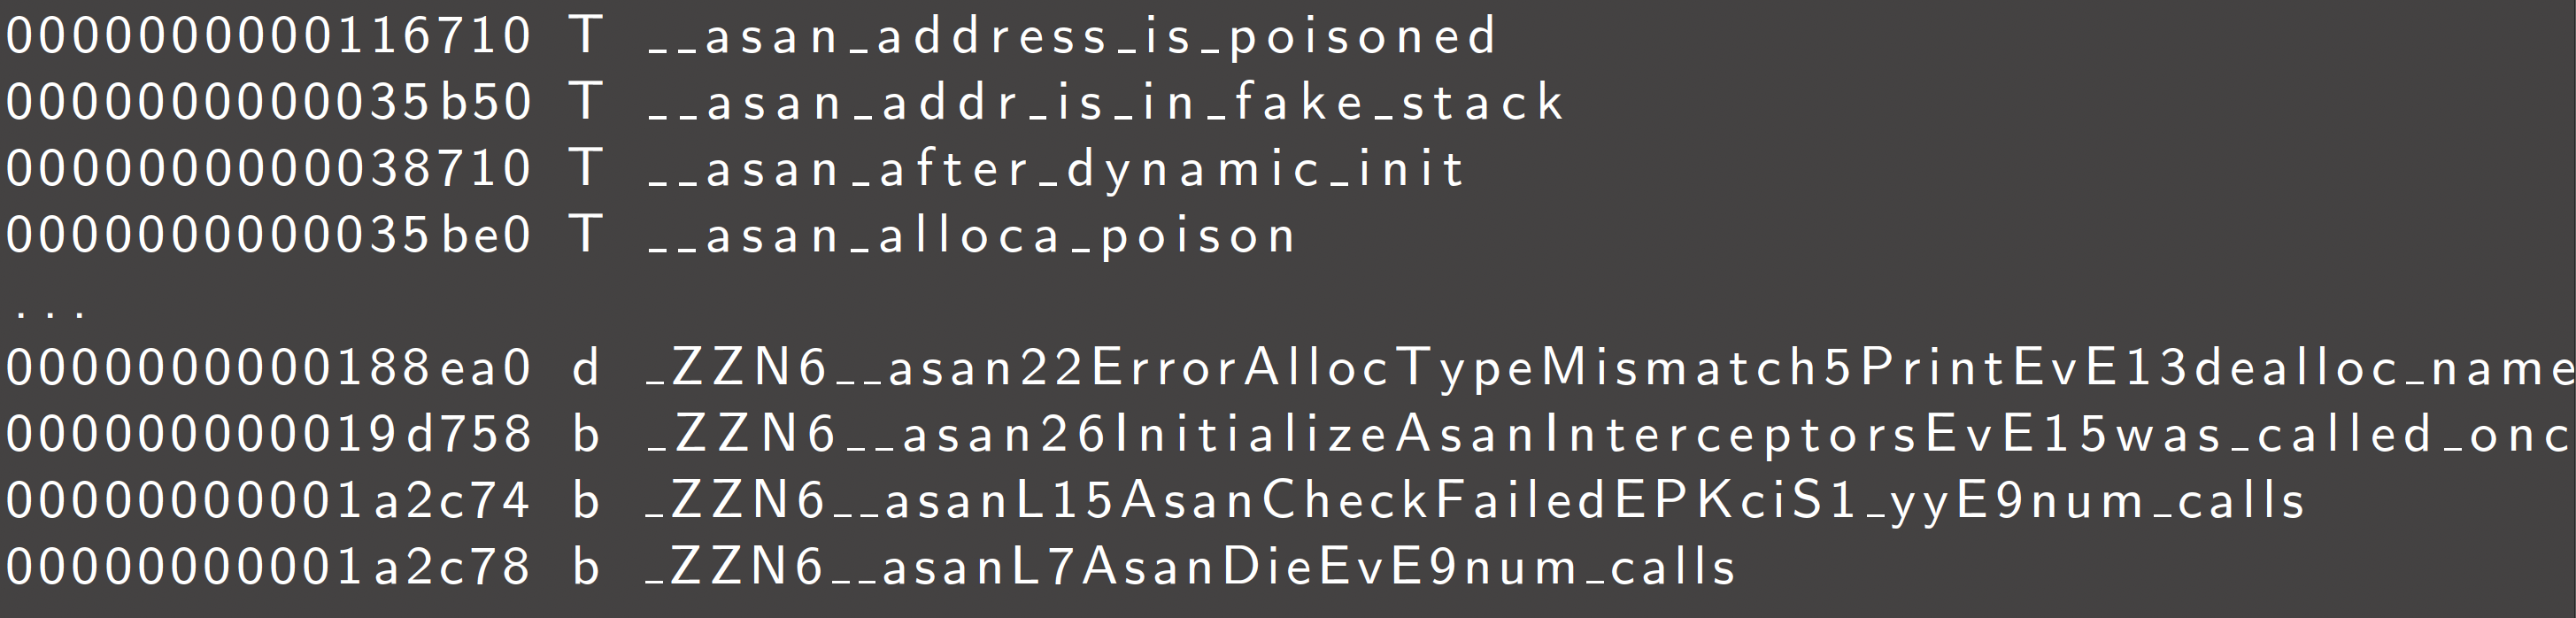
\includegraphics[width=.5\linewidth]{res/library_1.png}
    \caption{}
\end{figure}

\subsubsection{Dynamic linking}

Anche i file eseguibili possono sfruttare il linking, grazie a questa funzione la dimensione dei file diminuirà sensibilmente e si renderà molto più facile l'aggiornamento del codice.
Questo comportamento è impostato di default dal linker nei compilatori \textit{C} su linux.
\begin{figure}[h!]
    \centering
    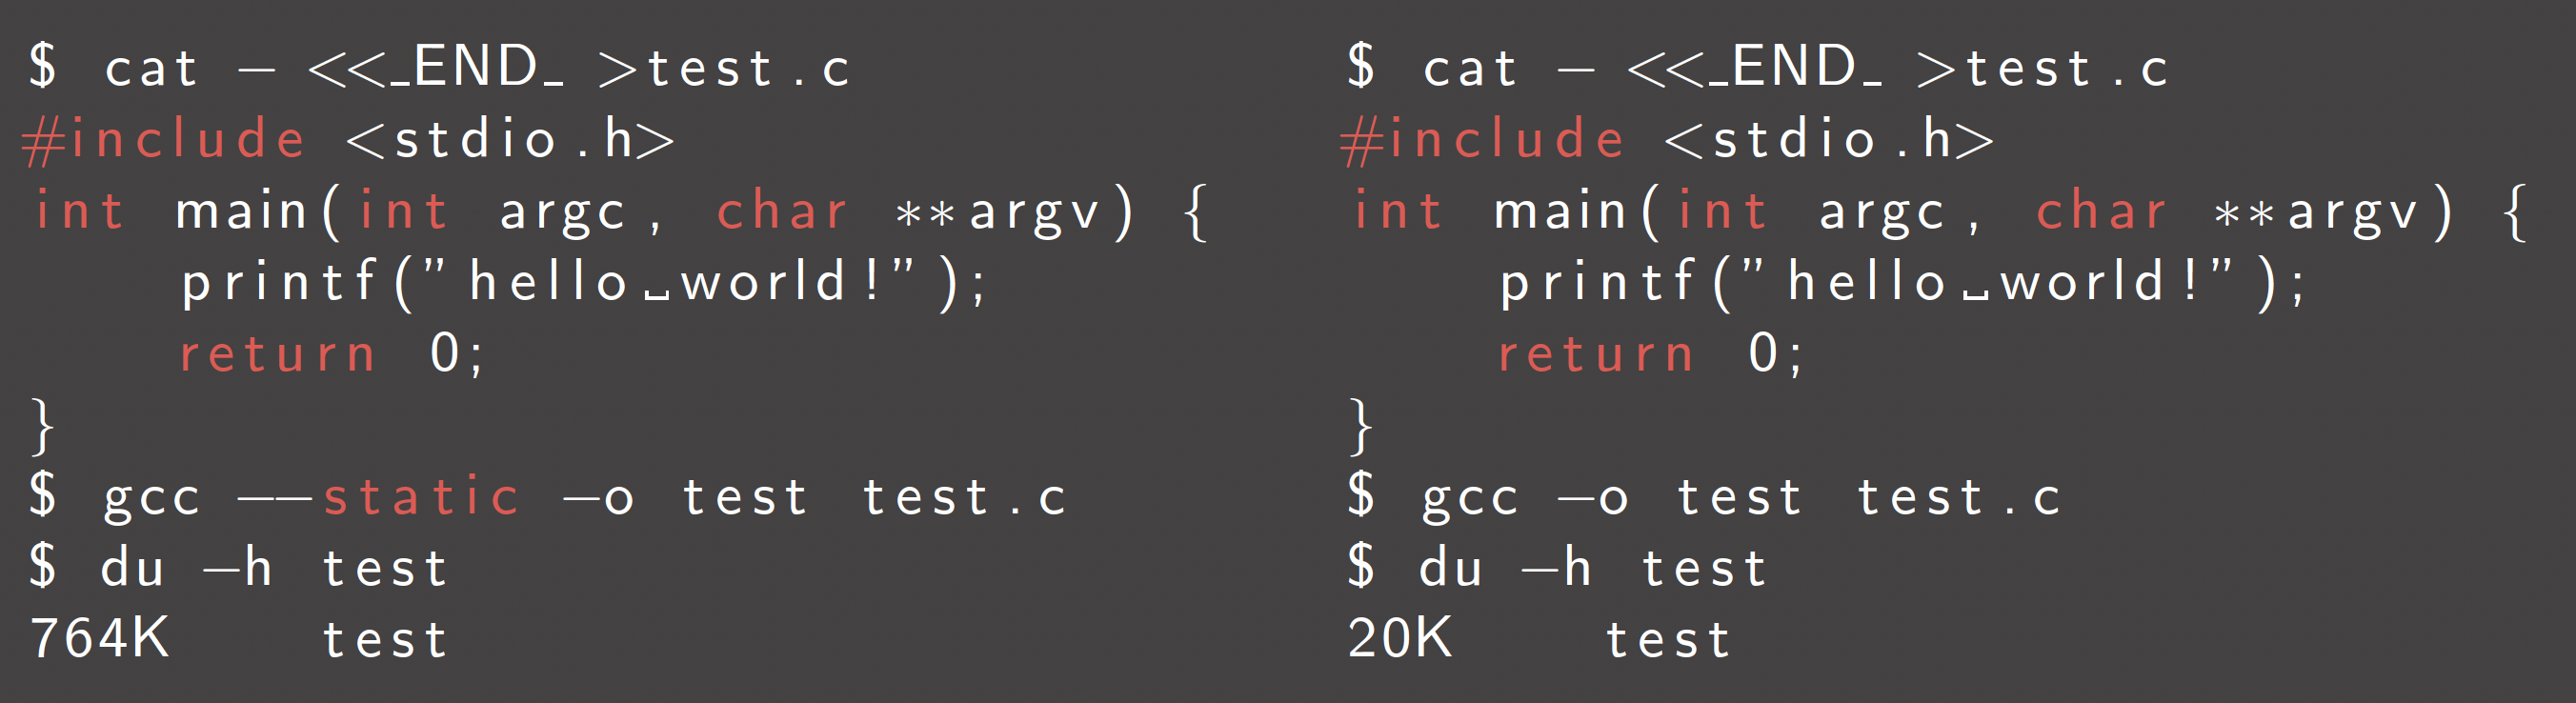
\includegraphics[width=.5\linewidth]{res/linking_2.png}
    \caption{}
\end{figure}
Come possiamo vedere nel secondo caso in cui le librerie non sono state importate in modo statico avremo una dimensione di molto inferiore rispetto al primo caso.
Quando il programma si trova ad eseguire il la sezione del loader (\textbf{.interp} section), si occuperà di caricare le librerie e aggiornare le referenze nel codice.
\begin{figure}[h!]
    \centering
    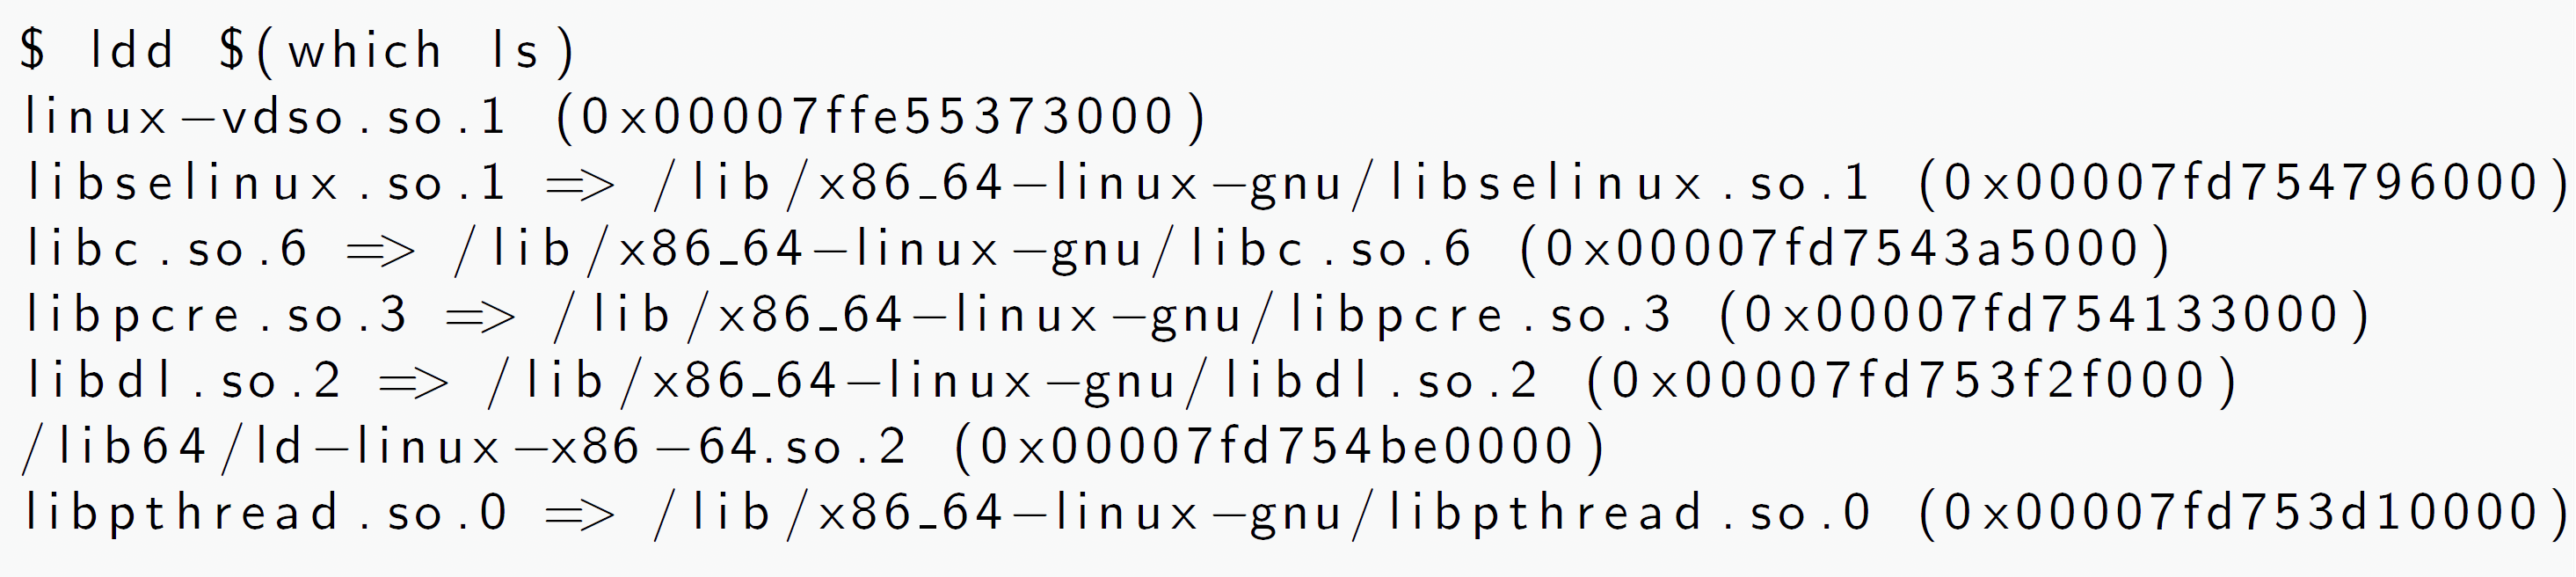
\includegraphics[width=.5\linewidth]{res/linking_3.png}
    \caption{}
\end{figure}

\subsubsection{Library hijacking}
Quando dichiara una libreria: 
\begin{lstlisting}[language=C]
    puts("ciao \n");
\end{lstlisting}
essa effettuerà un chiamata all'interno della libreria:
\begin{lstlisting}[language=bash]
    1154: e8 d7 fe ff ff callq 1030 <puts@plt> # @plt: chiamata per il linking dinamico
\end{lstlisting}
\textbf{Domanda:} É possibile effettuare un hijacking alla chiamata cambiando la libreria?

La risposta è si. Questa cosa si può effettuare a tempo di caricamento senza effettuare il relinking dell'applicazione.
\begin{lstlisting}[language=bash]
    $ ./test
    ciao
    $ LD_LIBRARY_PRELOAD= ./fakelib.so ./test
    hacked
\end{lstlisting}
utilizzando questa variabile d'ambiente si potrà effettuare l'hijack della libreria utilizzata in origine modificandone il comportamento delle funzioni di libreria.
Usando questo trick è possibile tracciare l'esecuzione del programma senza utilizzare i metodi convenzionali di debugging.

Supponiamo di avere i seguente codice:
\begin{lstlisting}[language=C]
    #include <stdio.h>
    #include <string.h>

    int main (int argc, char** argv) {
        if (argc < 2) {
            return 1;
        }

        if (!strcmp("super-secret-password", argv[1])) {
            print("Access granted!\n");
        }
        return 0;
    }
\end{lstlisting}
si potrà utilizare il comando \textbf{ltrace} per seguirne l'esecuzione:
\begin{lstlisting}[language=bash]
    command:
    ltrace ./test ciao

    output:
    strcmp("super-secure-password" , "ciao")               = 16
    +++ exited (status 0) +++       
\end{lstlisting}

\textbf{Domanda:} Cosa accade se utilizzassimo \textbf{LD\_LIBRARY\_PRELOAD} su un esecuzione privilegiata (setuid o ep capabilities).

I questo caso se l'eseguibile è privilegiato non verrà fatto hijacking.

\section{Kernel}
Il kernel è il programma che costituisce il cuore centrale del sistema operativo del computer. Ha il completo controllo su tutto ciò che accade nel sistema.
Si frappone tra il sistema operativo e l'hardware facendone da intermediario.

I tipi di kernel più utilizzati sono tre:
\begin{itemize}
    \item \textbf{Monolitici}, i kernel monoliti hanno un'integrazione del codice molto stretta tra i vari moduli, ciò potrebbe portare a un eventuale propagazione di qualche bug nel caso se ne presentasse uno;
    \item \textbf{Microkernel}, l'approccio a microkernel consiste nel definire un ristretto numero di primitive che si occupano di implementare i servizi minimali, sopra il kernel principale verranno innestati dei moduli che si occuperanno di implementare le altre funzioni attraverso le primitive del microkernel;
    \item \textbf{Ibridi}, l'approccio ibrido è di fatto un microkernel con del codice "non essenziale" implementato dentro di esso.
\end{itemize}
Noi ci focalizzeremo sui kernel monolitici, come linux o BSD. Il kernel è il responsabile di:
\begin{itemize}
    \item gestire il ciclo di vita dello spazio utenti (userland), processi;
    \item gestire le risorse
    \item interagire con l'hardware
    \item assicurare la sicurezza del sistema
\end{itemize}

Con il termine \textbf{userland} o user space, ci si riferisce a tutte quelle porzioni di codice che vengono eseguite al di fuori del kernel del sistema operativo. Probabilmente la maggior parte del codice che un programmatore scrive verrà eseguito proprio nello userland, al contrario del codice di un eventuale driver per qualche dispositivo che verrà eseguito nello spazio del kernel (kernel space).
\begin{figure}[h!]
    \centering
    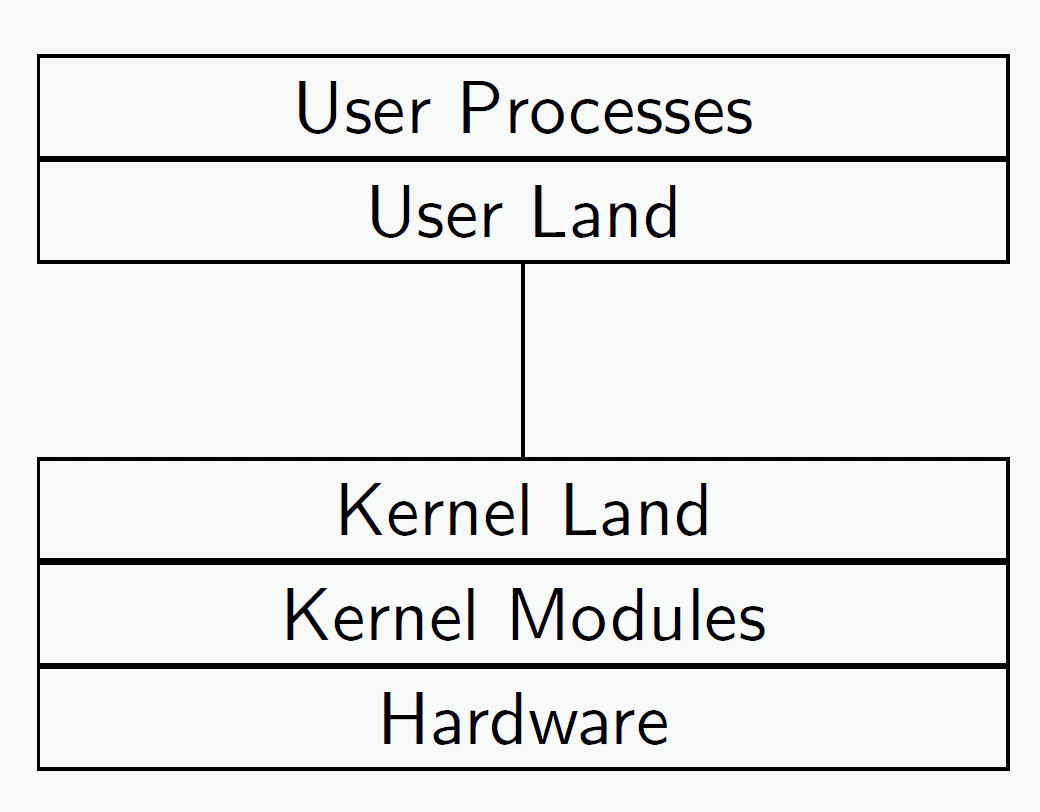
\includegraphics[width=.5\linewidth]{res/userland.png}
    \caption{}
\end{figure}
Riprendendo un concetto precedente, quello dei ring di sicurezza, potremo affermare che nel ring 3 vi sarà eseguito il codice dello userland mentre nel ring 0 sarà eseguito il codice del kernel space.

\section{Processi}
Un processo è un istanza di un programma, in linux i termini processo, task e thread sono qualche volta scambiati tra di loro.
In genere essi hanno questo significato:
\begin{itemize}
    \item \textbf{Task}, il compito di un processo, cosa vuole raggiungere e come;
    \item \textbf{Thread}, un istanza del programma, la memoria è condivisa tra i relativi threads di quel programma;
    \item \textbf{Process}, un contenitore di thread che condividono la stessa memoria.
\end{itemize}
In linux un thread e un processo sono la stessa cosa, un processo è un thread con la memoria separata dagli altri processi.

Un esempio lo possiamo trovare in due browser quali firefox e chrome, in firefox ogni tab è un thread al contrario di chrome in cui ogni tab è costituito da un processo.

\subsection{Process loading}
Quando un programma viene lanciato, l'interprete (loader) viene eseguito e il contenuto del file ELF viene caricato in memoria dalla MMU (.text, .rodata ecc.). La sezione .bss verrà inizializzata a 0 (mappata con una pagina vuota).
Le librerie dinamiche saranno altrettanto caricate in memoria e condivise attraverso i processi comuni.

\subsection{Segmented memory}
La memoria in un programma è segmentata similmente al file ELF, in questo caso il sistema caricherà le differenti aree, che comprendono anche l'acclocazione delle aree per la heap e per lo stack (allocate dall' MMU), in questa fase verranno anche protette le zone di memoria dando i relativi privilegi (esecuzione, scrittura, lettura).
\begin{figure}[h!]
    \centering
    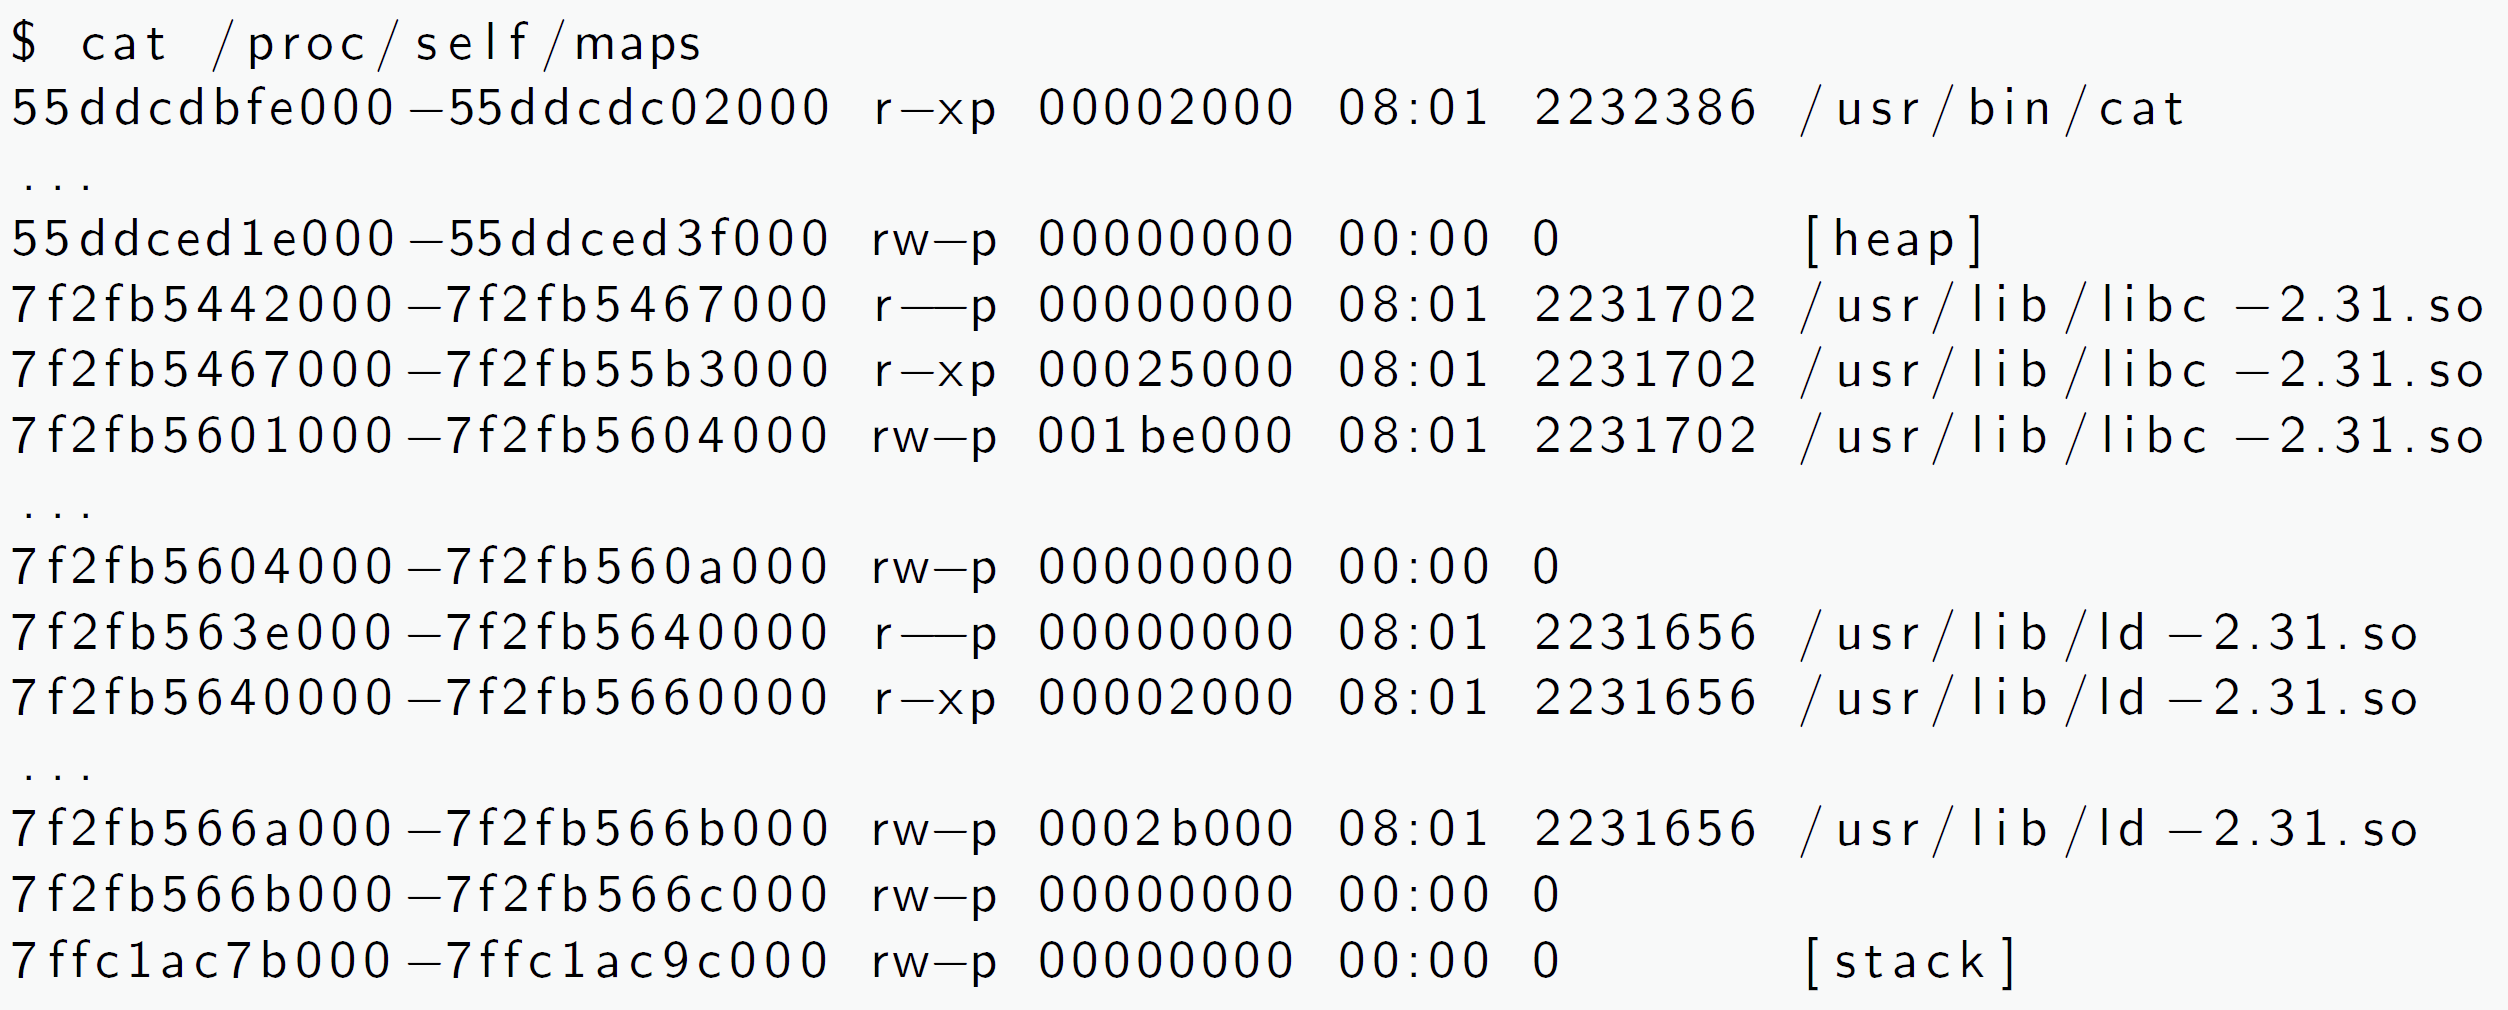
\includegraphics[width=.5\linewidth]{res/segmentation_memory.png}
    \caption{}
\end{figure}
\begin{lema}[]{}{}
    La locazione 0 (null) non è mappata in memoria centrale, ciò condurrà a un segmentation fault se acceduta.
\end{lema}

\section{Systemcall}
Una systemcall è una procedura che comunica con il kernel. Per risolvere la systemcall il sistema processerà la richiesta e opererà di conseguenza.
Alcune systemcall sono:
\begin{itemize}
    \item \textbf{open};
    \item \textbf{read};
    \item \textbf{write};
    \item \textbf{socket}.
\end{itemize}

Il sistema operativo deve accettare la procedura dal programma nello userland per ricevere i corretti parametri dallo userland.
Un esempio di x86\_32 bit: 
\begin{lstlisting}[language={[x86masm]Assembler}]
    int 0x80;
\end{lstlisting}
La trap può risultare troppo lenta, per questo è stato microprogrammato in un opcode dedicato nel x86\_64:
\begin{lstlisting}[language={[x86masm]Assembler}]
    syscall
\end{lstlisting}
Il valore della systemcall viene caricato nel registro \textit{rax} (\textit{eax} nei processori 32bit).
I parametri verranno passati nei seguenti registri:
\begin{itemize}
    \item \textit{\textbf{eax}};
    \item \textit{\textbf{ebx}};
    \item \textit{\textbf{ecx}};
    \item \textit{\textbf{edx}};
    \item \textit{\textbf{esi}};
    \item \textit{\textbf{edi}};
    \item \textit{\textbf{edp}};
\end{itemize}
mentre il codice di ritorno della systemcall sarà inviato all'utente attraversa il salvataggio nel registro \textit{rax} (\textit{eax} nei processori 32bit).
Per i sistemi a 64 bit i parametri saranno passati attraverso i registri:
\begin{itemize}
    \item \textit{\textbf{rdi}};
    \item \textit{\textbf{rsi}};
    \item \textit{\textbf{rdx}};
    \item \textit{\textbf{r10}};
    \item \textit{\textbf{r8}};
    \item \textit{\textbf{r9}};
\end{itemize}

A prima vista una systemcall può sembrare una chiamata ad una libreria, questa cosa è vera, ma seppur simili la libreria e la systemcall differiscono da lacune cose.
\begin{figure}[h!]
    \centering
    \begin{subfigure}{.5\textwidth}
      \centering
      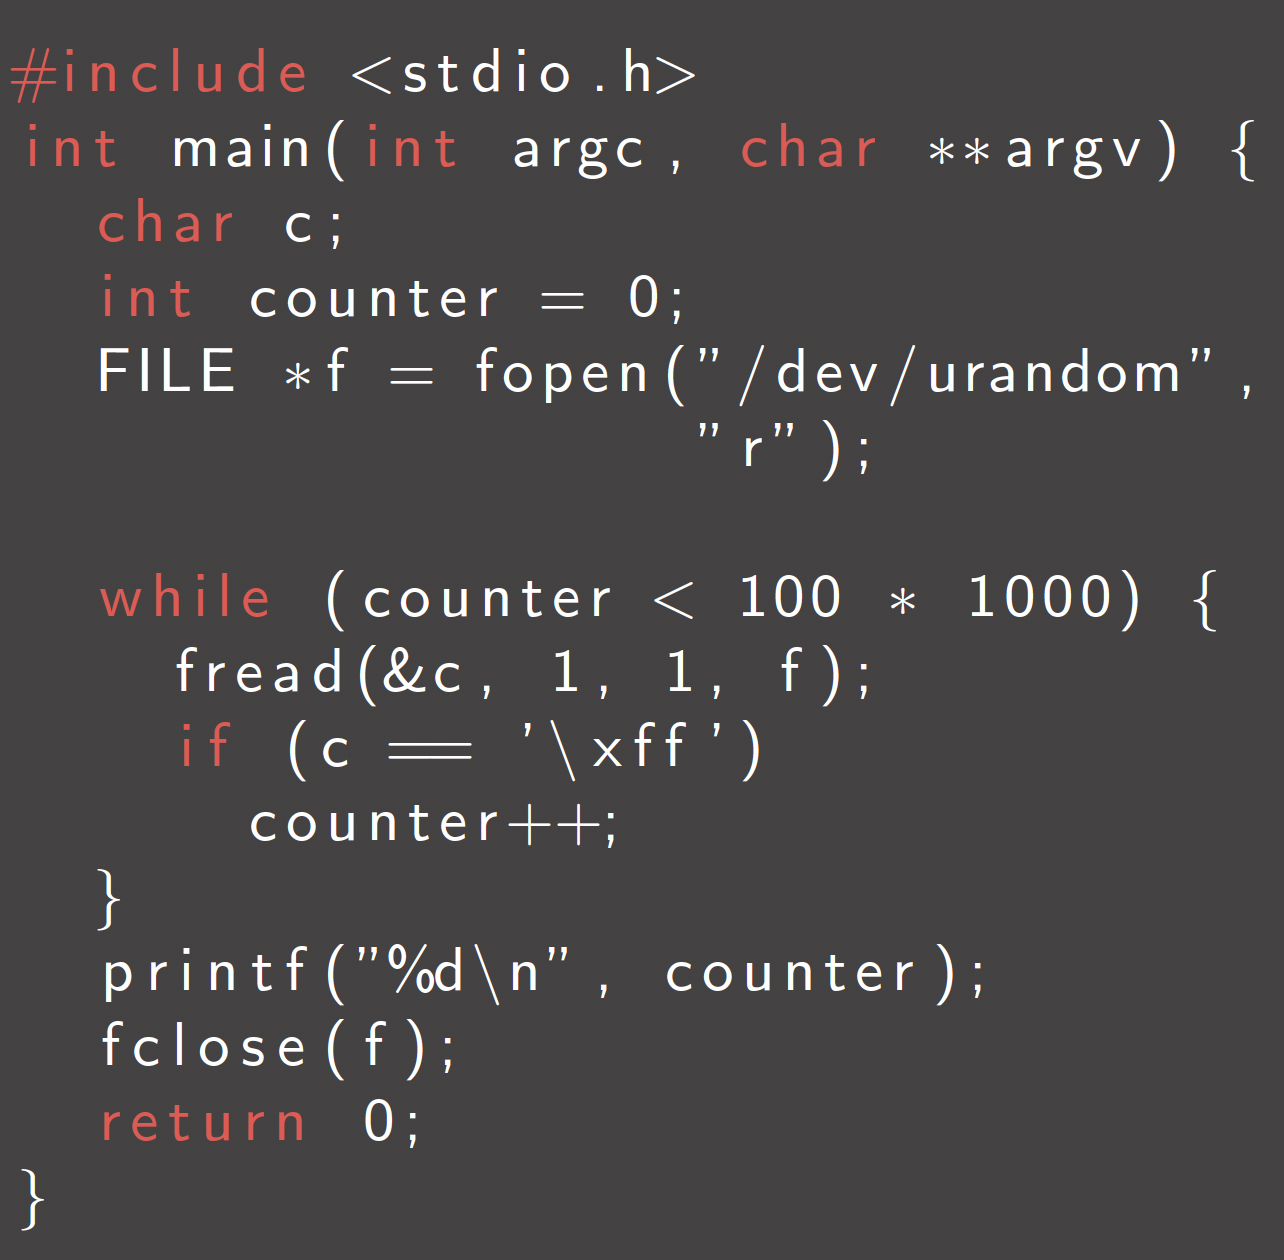
\includegraphics[width=.5\linewidth]{res/fopen_library.png}
      \caption{Utilizzo della libreria fopen}
    \end{subfigure}%
    \begin{subfigure}{.5\textwidth}
      \centering
      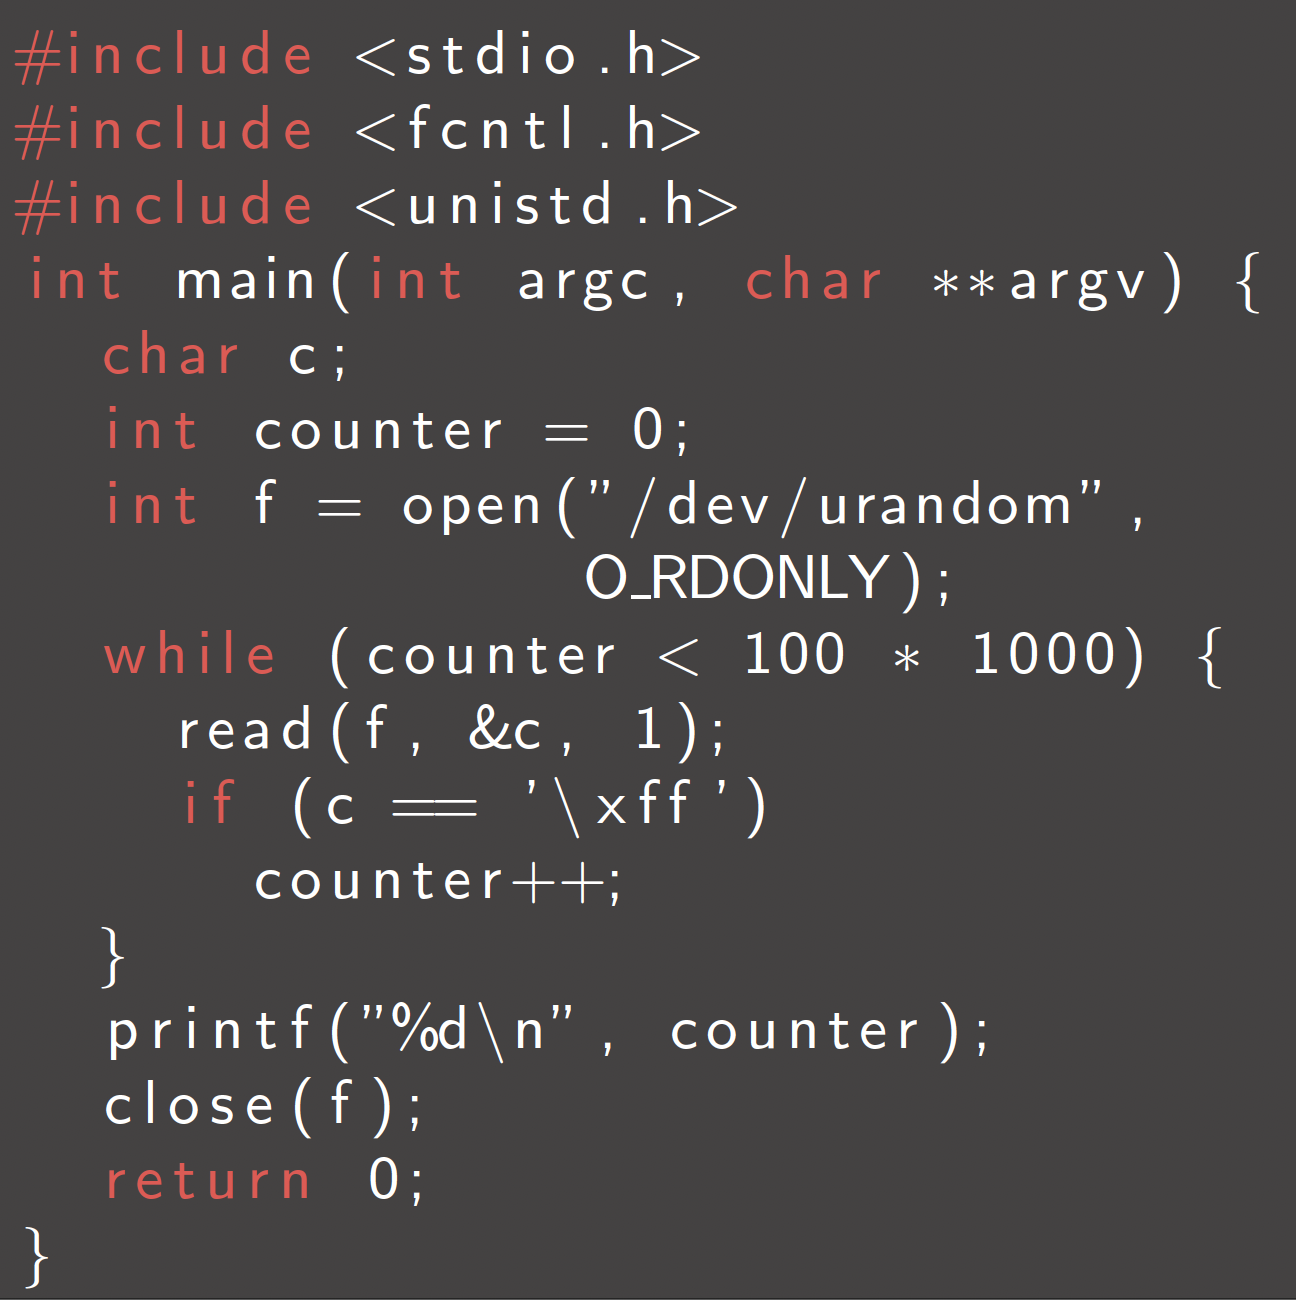
\includegraphics[width=.5\linewidth]{res/open_library.png}
      \caption{Utilizzo della syscall open}
    \end{subfigure}
\end{figure}

La differenza maggiore è nella velocità di esecuzione delle due, la syscall è sensibilmente più lenta di una libreria ottimizzata.
Infatti avremo che durante una syscall il trasferimento di dati sarà di un byte alla volta (\textit{read}), mentre nella libreria (\textit{fread}) la velocità sarà di una o più pagine alla volta, riducendo sensibilemnte il tempo di esecuzione.

Per come sono impelementate le systemcall avremo che ogni qual volta si effettuerà una lettura con \textit{read} avverrà un context switch, al contrario utilizzando \textit{fread} sarà letto un intero blocco di dati e trasferito byte per byte senza nessuno switch.

\subsection{Dynamic tracing}
\textit{\textbf{Ptrace}} è una systemcall in grado di controllare il comportamento di un programma tracciato. Può essere istruita per recuperare la memoria i registri e le systemcall invocate dal processo tracciato.
\begin{figure}[h!]
    \centering
    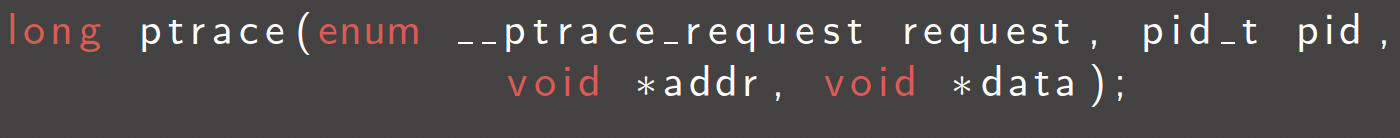
\includegraphics[width=.5\linewidth]{res/ptrace_header.png}
    \caption{}
\end{figure}
\textit{Strace} è un tool basato su \textit{Ptrace} che analizza dinamicamente un programma e stampa tutte le systemcall chiamate da esso.

\begin{figure}[h!]
    \centering
    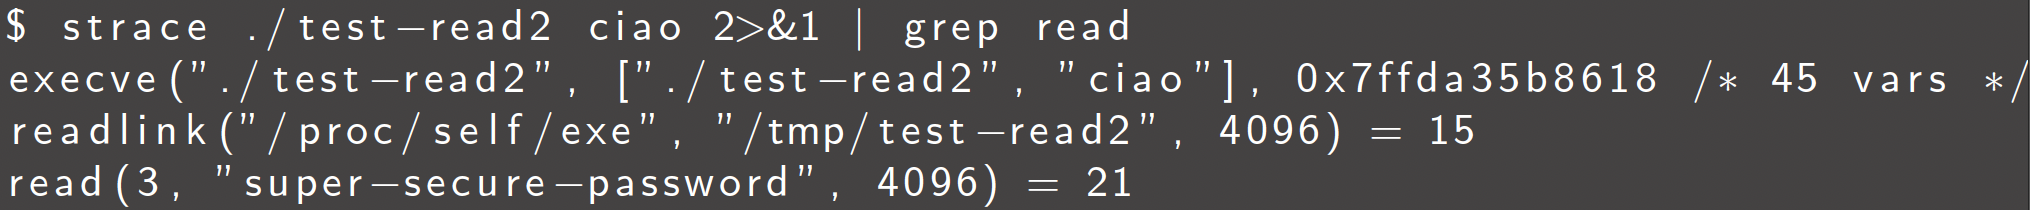
\includegraphics[width=.5\linewidth]{res/strace.png}
    \caption{}
\end{figure}

\subsection{Anti dynamic analysis}

Una delle tecniche di anti analisi dinamica è l'elusione di ptrace semplicemente tracciando se stesso e disabilitando il meccanismo di ptrace, come da manpage, in alcuni casi alcunelanguage virtual machines sono impiegate per offuscare il codice.

\begin{figure}[h!]
    \centering
    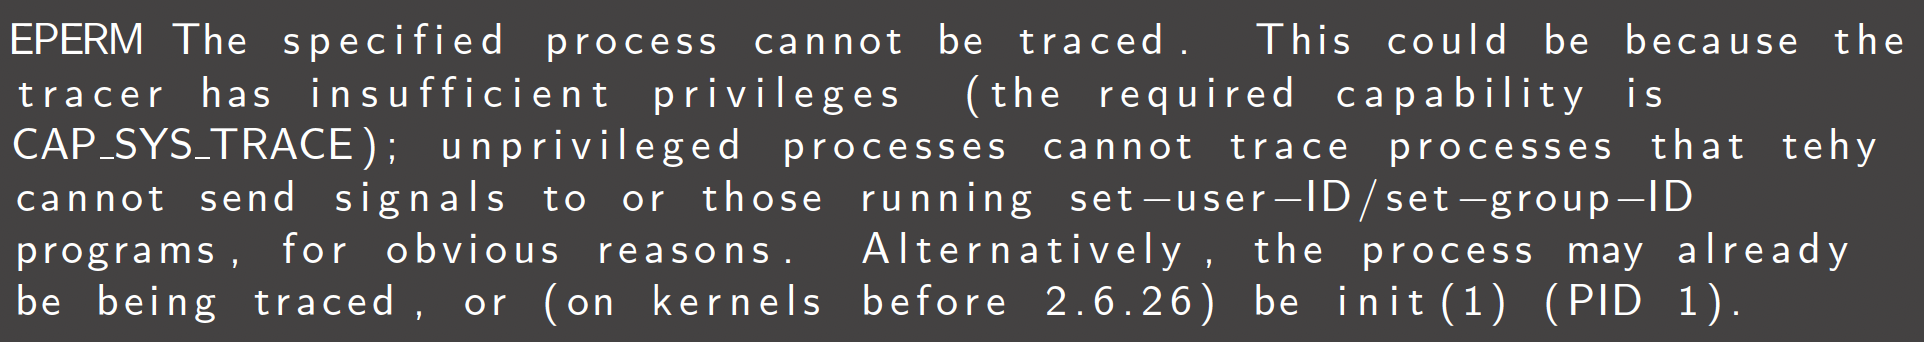
\includegraphics[width=.5\linewidth]{res/anti_analysis_ptrace.png}
    \caption{}
\end{figure}

Un altra tecnica impiegabile prende il nome di anti breakpoint, questa tecnica consiste nell'inserire l'opcode del debugger (\textit{0xcc}, int 3) che si usa per tracciare i breakpoint nei programmi.
In questo modo il programma puù controllare se sta essendo debuggato controllando la presenza di breakpoint, portando così un uscita prematura dal programma senza terminare la corretta esecuzione;

Supponiamo di avere il seguente codice:
\begin{lstlisting}[language=C]
    #include <stdio.h>
    #define PRINT_SIZE 16
    int foo() {
        unsigned char x = *(((unsigned char *)foo)+ 4);
        printf("%02x\n", x);
        if(x == 0xcc)
            printf("detected debugger! :D \n");
        return 0;
    }
    int main(int argc, char **argv) {
        foo();
        return 0;
    }
\end{lstlisting}

\begin{figure}[h!]
    \centering
    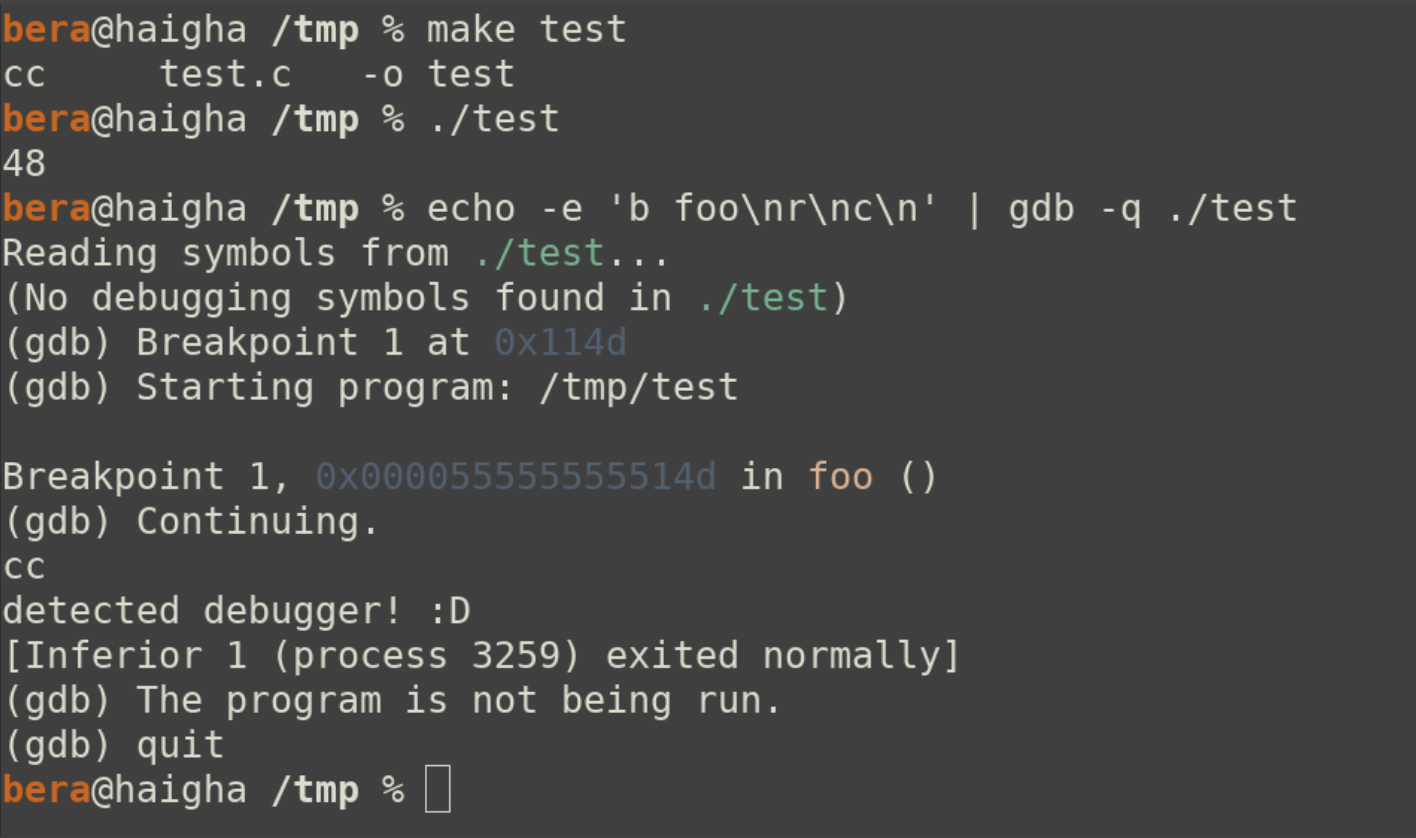
\includegraphics[width=.5\linewidth]{res/anti_breakpoint.png}
    \caption{}
\end{figure}

\subsection{Systemcall firewalls}
Le systemcall possono essere inserite in una tabella di firewall in linux utulizzando BGP, possono essere caricate nella seguente maniera:
\begin{itemize}
    \item \textbf{BPF} (Berkeley packet filter);
    \item \textbf{Plege}, e altre implementazioni.
\end{itemize}

\subsubsection{BPF (Berkeley packet filter)}
É language virtual machine inserita nel kernel linux atta a velocizzare le operazioni di filtraggio dei firewalls. Questo linguagio specifica le regole che accettano o rifiutano un pacchetto.
In questo caso i parametri delle systemcall sono mappati come campi dei pacchetti, in questo modo la systemcall può essere filtrata dal programma che la invoca, limitatamente al set delle systemcall utilizzabili.

\subsubsection{Plege}
Alcuni kernel hanno una differe implementazione di questo concetto come \textbf{pledge(2)} in OpenBSD.
Essa verrà trattata nelle successive lezioni. Si può immaginare comunque a un firewall che blocca le systemcall di ptrace, in questo caso l'uso di GDB sarà bloccato dal firewall stesso.

\section{Modifiche statiche di un binario}
Sappiamo modificare il comportamento dinamico di un programma, ma cosa sappiamo del comportamento statico di un binario?
Possiamo alterarne il codice inserendo diversi opcode tramite l'uso di tool di base come vim o xxd.

Prendiamo in esempio questo codice:
\begin{lstlisting}[language=C]
    #include <stdio.h>
    #include <string.h>
    int main(int argc, char **argv){
        char buf[8];
        FILE *f;
        if (argc < 2)
            return 1;
        f = fopen("/dev/urandom", "r");
        fread(buf, 1, sizeof(buf), f);
        fclose(f);
        if(!memcmp(buf, argv[1], sizeof(buf)))
            printf("Wow!\n");
        return 1;
    }    
\end{lstlisting}

otterremo questo codice assembly:
\begin{figure}[h!]
    \centering
    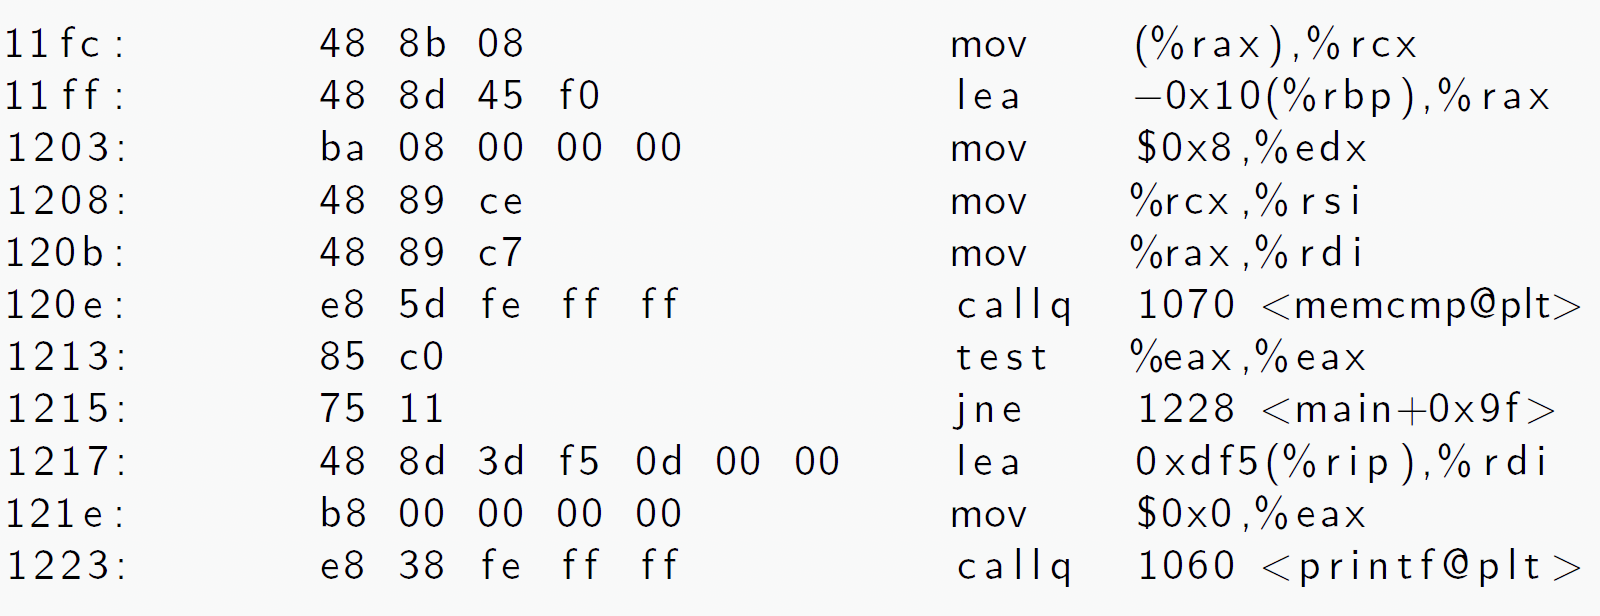
\includegraphics[width=.6\linewidth]{res/static_modification_test.png}
    \caption{}
\end{figure}

Osservando il codice possiamo notare la riga con il comando \textit{jne} (0x75), cosa succederebbe se la modificassimo in \textit{je} (0x74)?
\begin{figure}[h!]
    \centering
    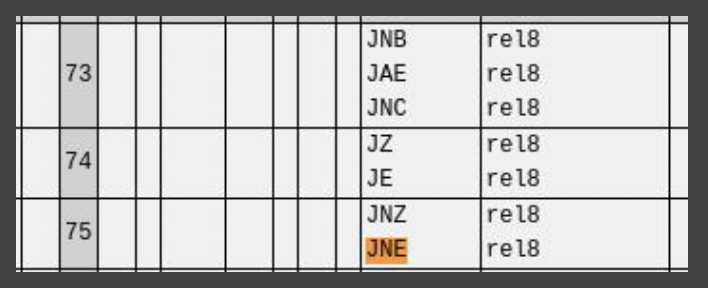
\includegraphics[width=.6\linewidth]{res/jump_table_code.png}
    \caption{}
\end{figure}

utilizzando il tool xxd potremo effettuare questa modifica come segue:
\begin{lstlisting}[language=bash]
    xxd -PS test > test.hex
    sed -i 's/ffff85c07511/ffff85c07411/' test.hex
    xxd -ps -r test.hex > test
\end{lstlisting}

otterremo il seguente risultato:
\begin{figure}[h!]
    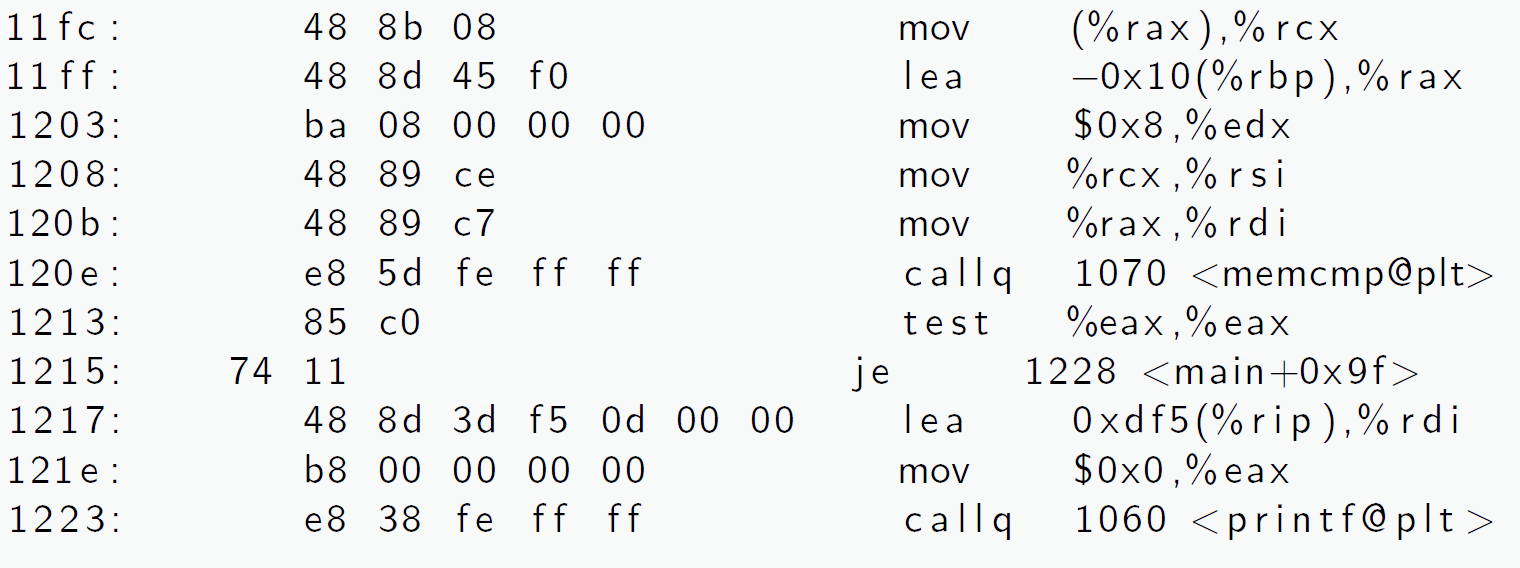
\includegraphics[width=.6\linewidth]{res/static_modificatio_test2.png}
    \centering
    \caption{}
\end{figure}
adesso potremo eseguire il programma e avremo una bella sorpresa:
\begin{lstlisting}[language=bash]
    command:
    ./test ciao

    output:
    Wow!
\end{lstlisting}
potremo vedere come il controllo non sia stato effettuato e quindi siamo riusciti ad eluderlo per farci stamapare ciò che volevamo.

\begin{lema}
    Il cambio di codice effettuato ha dei limiti in quanto in base all'architettura (e.g. x86\_64) dovremo controllare il comando da inserire sia al massimo grande quanto quello da modificare nel caso in cui i byte siano variabili perchè altrimenti andremo a sovrascrivere altri byte portando a un errore in esecuzione.
    Questa cosa non avviene nel caso in cui il byte siano fissati perchè ogni comando avrà semore quello spazio a disposizione a prescindere se più piccolo, se un comando risualta più corto è consigliato inserire il codice di \textit{NOP (0x90)} (ignora l'istruzione e va avanti) per evitare di sporcare la memoria e rendere alterata l'esecuzione.
    Questa modalità prende il nome di NOP Sled perchè permette anche di indirizzare l'esecuzine verso il nostro shellcode senza conoscerne precisamente la posizione in memoria.
\end{lema}

Un altro metodo per effettuare l'analisi statica è quella di utilizzare il framework \textit{angr} (combina l'analisi statica e dinamica simbolica, concolic analysis).
Utilizzando questo framework l'eseguibile verrà caricato nel framework, successivamente il binario verrà trasformato in \textbf{IR} (intermediate representation) e infine verrà eseguita l'analisi.
